\documentclass[11pt,a4paper]{article}
\usepackage[margin=1in]{geometry}
\usepackage{amsmath,amssymb,amsthm,mathtools}
\usepackage{microtype}
\usepackage{parskip}
\usepackage{enumitem}

\usepackage{placeins} 

\usepackage{pgfplots}
\pgfplotsset{compat=1.18}

\usepackage{tikz}
\usepackage{graphicx}
\usepackage{array}

\usepackage{float}

\usepackage{varwidth} % add if not already in preamble
\usepackage[most]{tcolorbox}
\tcbuselibrary{theorems}

\usepackage[colorlinks=true,linkcolor=blue]{hyperref} % optional but recommended
\usepackage[capitalize,nameinlink,noabbrev]{cleveref}


\usetikzlibrary{arrows.meta}
\usepgfplotslibrary{groupplots}

\newtheorem{theorem}{Theorem}
\newtheorem{example}{Example}
\newtheorem{counterexample}{Counterexample}
\newtheorem{corollary}[theorem]{Corollary}
\theoremstyle{definition}
\newtheorem{exercise}{Exercise} % or [subsection] or no bracket for global numbering

\usepackage{enumitem}



\usepackage[most]{tcolorbox} % loads skins + breakable
\tcbuselibrary{theorems}

\usetikzlibrary{arrows.meta,decorations.markings}

% definition style (not italic)
\theoremstyle{definition}

\newtheorem{definition}[exercise]{Definition}

% plain style (italic body)
\theoremstyle{plain}

\newtheorem{lemma}[exercise]{Lemma}

% remark style (upright text, not italic)
\theoremstyle{remark}
\newtheorem{remark}[exercise]{Remark}

\DeclareMathOperator{\Log}{Log}
\DeclareMathOperator{\Arg}{Arg} 
\DeclareMathOperator{\Res}{Res}

\newcommand{\DrawDyadicInterpolant}[3]{% #1=M, #2=expr in \x, #3=plot options
	\pgfmathtruncatemacro{\N}{2^#1}
	\addplot+[#3] coordinates {%
		\foreach \j in {0,...,\N}{%
			\pgfmathsetmacro{\x}{\j/\N}
			\pgfmathsetmacro{\y}{#2}%
			(\x,\y)
		}%
	};
}

% Faber–Schauder hat: \varphi_{m,k}(t)=max(1-2^{m+1}|t-k/2^m|,0)
\newcommand{\DrawHat}[3]{% #1=m (>=1), #2=k odd, #3=plot options
	\addplot+[domain=0:1,samples=400,#3]
	{max(1 - abs((2^(#1))*x - (#2)), 0)};
}





% a matching solution environment
%\newenvironment{solution}{\begin{proof}[Solution]}{\end{proof}}

\emergencystretch=2em
\setlength{\abovedisplayskip}{9pt}
\setlength{\belowdisplayskip}{9pt}
\setlength{\abovedisplayshortskip}{7pt}
\setlength{\belowdisplayshortskip}{7pt}

\newcommand{\norm}[1]{\left\lVert #1 \right\rVert}
\newcommand{\Pspace}{\mathcal{P}_{<n}}
\newcommand{\Err}{E^\ast_n}


\usepackage{amsthm}
\newtheorem{problem}{Problem}[section] % or omit [section] if you don't want section-based numbering
\newenvironment{solution}{\par\noindent\textbf{Solution.}\ }{\hfill\qedsymbol\par}



\newtheorem{proposition}[theorem]{Proposition}

%\newenvironment{solution}{\par\noindent\textit{Solution.}\ }{\par\vspace{0.5em}}

% === Adjusted title info ===
\title{Exercises and Solutions \\[0.5em]
	\large Theory of Complex analysis}
\author{Prepared by \dots}
\date{\today}

\begin{document}
	\maketitle
	
	
\section*{Real-linear maps $\mathbb{R}^2\!\to\!\mathbb{R}^2$ viewed as $\mathbb{C}\to\mathbb{C}$}

\begin{problem}\label{prob:real-linear-C-decomp}
	Let $T:\mathbb{R}^2\to\mathbb{R}^2$ be a real-linear map. Regard $T$ as a map $\mathbb{C}\to\mathbb{C}$ via $(x,y)\leftrightarrow x+iy$.
	Show that there exist unique $A,B\in\mathbb{C}$ such that
	\[
	T(z)=Az+B\overline{z}\qquad(\forall\,z\in\mathbb{C}),
	\]
	and that $T$ is complex differentiable (i.e.\ $\mathbb{C}$-linear) iff $B=0$.
\end{problem}



\subsection*{Background and definitions}
\begin{itemize}
	\item A map $T:\mathbb{C}\to\mathbb{C}$ is \emph{real-linear} if
	$T(\alpha z+\beta w)=\alpha T(z)+\beta T(w)$ for all $z,w\in\mathbb{C}$ and all \emph{real} $\alpha,\beta$.
	\item It is \emph{complex-linear} (holomorphic and linear) if the same holds for complex $\alpha,\beta$, equivalently $T(iz)=iT(z)$ for all $z$.
	\item Every $z=x+iy$ has the conjugate $\bar z=x-iy$. Note that $x=\frac{z+\bar z}{2}$ and $y=\frac{z-\bar z}{2i}$.
	\item The \emph{Wirtinger operators} are
	$\displaystyle \frac{\partial}{\partial z}=\frac12\!\left(\frac{\partial}{\partial x}-i\frac{\partial}{\partial y}\right)$ and
	$\displaystyle \frac{\partial}{\partial \bar z}=\frac12\!\left(\frac{\partial}{\partial x}+i\frac{\partial}{\partial y}\right)$.
	A $C^1$ map $F$ is holomorphic iff $\partial F/\partial\bar z=0$.
\end{itemize}

\subsection*{Solution}
\textbf{Existence.}
Let $\alpha:=T(1)$ and $\beta:=T(i)$, viewed as complex numbers.
Seek $A,B\in\mathbb{C}$ with $T(z)=Az+B\bar z$. Then
\[
\alpha=T(1)=A+B,\qquad \beta=T(i)=A\,i+B\,\overline{i}=i(A-B).
\]
Solve
\[
A+B=\alpha,\qquad A-B=-\,i\,\beta
\quad\Longrightarrow\quad
A=\frac{\alpha-i\beta}{2},\qquad B=\frac{\alpha+i\beta}{2}.
\]
Define $A,B$ by these formulas. For any $z=x+iy$,
\[
Az+B\bar z
= A(x+iy)+B(x-iy)
= (A+B)x + i(A-B)y
= \alpha x + \beta y
= T(x)+T(iy)=T(z),
\]
since $T$ is real-linear. Hence $T(z)=Az+B\bar z$ for all $z$.

\smallskip
\textbf{Uniqueness.}
If $Az+B\bar z=A'z+B'\bar z$ for all $z$, then plugging $z=1$ and $z=i$ gives
$A+B=A'+B'$ and $i(A-B)=i(A'-B')$, hence $A=A'$ and $B=B'$.

\smallskip
\textbf{Complex differentiability $\iff B=0$.}
If $B=0$, then $T(z)=Az$ is complex-linear (multiplication by $A$), hence holomorphic.
Conversely, if $T$ is complex-linear, then $T(i)=iT(1)$, i.e.\ $\beta=i\alpha$.
From the formulas above,
\[
B=\frac{\alpha+i\beta}{2}=\frac{\alpha+i(i\alpha)}{2}=\frac{\alpha-\alpha}{2}=0.
\]
Equivalently, writing $T(z)=u(x,y)+iv(x,y)$, one computes
\[
\frac{\partial T}{\partial\bar z}=B,
\]
so the Cauchy–Riemann condition $\partial T/\partial\bar z=0$ is exactly $B=0$.

\qed

\subsection*{Concrete formulas in terms of a real matrix}
If $T$ has real matrix $\begin{psmallmatrix}a&b\\ c&d\end{psmallmatrix}$ so that
$T(x+iy)=(ax+by)+i(cx+dy)$, then
\[
A=\frac{a+d}{2}+i\,\frac{c-b}{2},\qquad
B=\frac{a-d}{2}+i\,\frac{c+b}{2}.
\]
Thus $T$ is complex-linear iff $b=-c$ and $a=d$ (i.e.\ the matrix is
$\begin{psmallmatrix}a&-t\\ t&a\end{psmallmatrix}$, multiplication by $a+it$).

\subsection*{Examples}
\begin{enumerate}
	\item \textbf{Identity:} $T(z)=z$. Here $A=1$, $B=0$ (holomorphic).
	\item \textbf{Rotation-scaling:} $T(z)=\lambda z$ with $\lambda\in\mathbb{C}$. Then $A=\lambda$, $B=0$ (holomorphic).
	\item \textbf{Complex conjugation:} $T(z)=\bar z$. Here $A=0$, $B=1$ (not holomorphic).
	\item \textbf{Real projection:} $T(z)=\mathrm{Re}(z)=\frac{z+\bar z}{2}$. Then $A=B=\frac12$ (not holomorphic).
	\item \textbf{General linear example:}
	$T(x+iy)=(2x+y)+i(3x-4y)$ has
	$A=\frac{2-4}{2}+i\frac{3-1}{2}=-1+i,\quad
	B=\frac{2+4}{2}+i\frac{3+1}{2}=3+2i$ (not holomorphic since $B\neq0$).
\end{enumerate}

\subsection*{Remarks}
The decomposition $T(z)=Az+B\bar z$ is the \emph{polarization} of real-linear maps.
The coefficient $A=\partial T/\partial z$ is the complex (holomorphic) part and
$B=\partial T/\partial\bar z$ is the antiholomorphic part. Holomorphic linear maps
are exactly those with vanishing antiholomorphic part.

\subsection*{Exercises on $T(z)=Az+B\bar z$ (with solutions)}

\begin{enumerate}
	\item (\textbf{Recover $A,B$ from a real matrix})  
	Let $T$ have real matrix $\begin{psmallmatrix}a&b\\ c&d\end{psmallmatrix}$ via
	$T(x+iy)=(ax+by)+i(cx+dy)$. Derive $A,B$ in $T(z)=Az+B\bar z$.
	
	\emph{Solution.} Compare coefficients using $z=x+iy,\ \bar z=x-iy$:
	\[
	A=\frac{a+d}{2}+i\,\frac{c-b}{2},\qquad
	B=\frac{a-d}{2}+i\,\frac{c+b}{2}.
	\]
	
	\item (\textbf{Quick diagnostics})  
	For each matrix, compute $(A,B)$ and decide if $T$ is complex-linear.
	\[
	\text{(a) }\begin{psmallmatrix}2&1\\ -1&2\end{psmallmatrix}\quad
	\text{(b) }\begin{psmallmatrix}1&1\\ 1&1\end{psmallmatrix}\quad
	\text{(c) }\begin{psmallmatrix}0&1\\ 1&0\end{psmallmatrix}.
	\]
	\emph{Solution.}
	(a) $A=2+i(-1-1)/2=2-i,\ B=\tfrac{2-2}{2}+i\tfrac{-1+1}{2}=0$ $\Rightarrow$ holomorphic.  
	(b) $A=1+i\,0=1,\ B=0+i\,1=i$ $\Rightarrow$ not holomorphic.  
	(c) $A=\tfrac{0+0}{2}+i\,\tfrac{1-1}{2}=0,\ B=\tfrac{0-0}{2}+i\,\tfrac{1+1}{2}=i$ $\Rightarrow$ not holomorphic.
	
	\item (\textbf{Matrix from $A,B$})  
	Given $T(z)=Az+B\bar z$ with $A=\alpha+i\beta$, $B=\gamma+i\delta$ ($\alpha,\beta,\gamma,\delta\in\mathbb{R}$), show the real matrix is
	\[
	\begin{pmatrix}
		\alpha+\gamma & -\beta+\delta\\
		\beta+\delta & \alpha-\gamma
	\end{pmatrix}.
	\]
	\emph{Solution.} Expand $Az+B\bar z$ with $z=x+iy$ and collect $(x,y)$ coefficients.
	
	\item (\textbf{CR in matrix form})  
	Show $T$ is complex-linear iff $a=d$ and $b=-c$.  
	\emph{Solution.} From Ex.\ 1, $B=0\iff a=d,\ c=-b$, i.e.\ matrix $\begin{psmallmatrix}a&-t\\ t&a\end{psmallmatrix}$.
	
	\item (\textbf{Wirtinger derivatives})  
	For $T(z)=Az+B\bar z$, compute $\partial T/\partial z$ and $\partial T/\partial\bar z$.  
	\emph{Solution.} $\displaystyle \frac{\partial T}{\partial z}=A,\qquad \frac{\partial T}{\partial\bar z}=B$.
	
	\item (\textbf{Composition law})  
	Let $T(z)=Az+B\bar z$ and $S(z)=Cz+D\bar z$. Show
	\[
	S\circ T(z)=(CA+D\overline{B})\,z\;+\;(CB+D\overline{A})\,\bar z.
	\]
	Deduce that the set of real-linear maps $\mathbb{C}\to\mathbb{C}$ is closed under composition, and $S\circ T$ is complex-linear iff $CB+D\overline{A}=0$.
	\emph{Solution.} Note $\overline{T(z)}=\overline{A}\bar z+\overline{B}z$ and compute
	$S(T(z))=C\,T(z)+D\,\overline{T(z)}$; read off the $z,\bar z$ coefficients.
	
	\item (\textbf{Jacobian, determinant, and orientation})  
	Show the Jacobian determinant of $T$ equals
	\[
	\det DT=|A|^2-|B|^2.
	\]
	Conclude that $T$ is orientation-preserving iff $|A|>|B|$, reversing iff $|A|<|B|$, and singular iff $|A|=|B|$.
	
	\emph{Solution.} Using Ex.\ 3’s matrix and a short computation:
	$\det=\!(\alpha+\gamma)(\alpha-\gamma)-(-\beta+\delta)(\beta+\delta)
	=(\alpha^2+\beta^2)-(\gamma^2+\delta^2)=|A|^2-|B|^2$.
	
	\item (\textbf{Operator norm and singular values})  
	Show the maximal and minimal stretch factors (singular values) of $T$ are
	\[
	\sigma_{\max}=|A|+|B|,\qquad \sigma_{\min}=\bigl||A|-|B|\bigr|.
	\]
	\emph{Solution (sketch).} Write $T(z)=A\bigl(z+\tfrac{B}{A}\bar z\bigr)$ if $A\neq0$; by rotating/scaling the domain and range one reduces to $A\ge0$, $B\ge0$ real. Then $T$ acts by stretching along two orthogonal directions with factors $A\pm B$, giving the claim. General case follows by unitary conjugation.
\end{enumerate}

\subsection*{Worked examples and illustrations}

\paragraph{Example A (Rotation–scaling; holomorphic).}
Let $T(z)=\lambda z$ with $\lambda=1.3 e^{i\pi/6}$. Then $A=\lambda$, $B=0$.
The image of the unit circle is a circle of radius $1.3$ rotated by $\pi/6$, and $T$ preserves angles and orientation.

\paragraph{Example B (Conjugation).}
Let $T(z)=\bar z$. Then $A=0$, $B=1$.
The unit circle is fixed as a set, but orientation is reversed. $T$ is not complex-differentiable since $B\neq0$.

\paragraph{Example C (Real shear).}
Let $T$ have real matrix $\begin{psmallmatrix}1&1\\ 0&1\end{psmallmatrix}$.
By the formulas,
\[
A=\frac{1+1}{2}+i\,\frac{0-1}{2}=1-\tfrac{i}{2},\qquad
B=\frac{1-1}{2}+i\,\frac{0+1}{2}=\tfrac{i}{2}.
\]
The image of the unit circle is an ellipse tilted by the shear. Since $B\neq0$, $T$ is not holomorphic.
The Jacobian is $|A|^2-|B|^2=(1^2+(\tfrac12)^2)-(\tfrac12)^2=1>0$, so orientation is preserved.

\paragraph{Example D (General mixed map).}
Take $A=1+\tfrac12 i$, $B=0.6-0.2i$. Then
\[
\det DT=|A|^2-|B|^2=(1^2+\tfrac{1}{4})-(0.6^2+0.2^2)=1.25-0.40=0.85>0,
\]
so $T$ is invertible and orientation-preserving, but not holomorphic ($B\neq0$).
Singular values are $\sigma_{\max}=|A|+|B|\approx \sqrt{1.25}+ \sqrt{0.40}$ and
$\sigma_{\min}=||A|-|B||$, giving principal stretches of the ellipse.

\begin{figure}[h]
	\centering
	
\includegraphics[width=.45\linewidth]{figures/Downloads_example_rotation_scaling.png}\hfill
	
\includegraphics[width=.45\linewidth]{figures/Downloads_example_conjugation.png}
	\caption{Left: $T(z)=1.3e^{i\pi/6}z$ (holomorphic). Right: $T(z)=\bar z$ (orientation-reversing).}
\end{figure}

\begin{figure}[h]
	\centering
	
\includegraphics[width=.45\linewidth]{figures/Downloads_example_shear.png}\hfill
	
\includegraphics[width=.45\linewidth]{figures/Downloads_example_general_mixed.png}
	\caption{Left: real shear $[[1,1],[0,1]]$. Right: general mixed case $A=1+0.5i$, $B=0.6-0.2i$.}
\end{figure}

\paragraph{Notes.}
For any $T(z)=Az+B\bar z$, the image of the unit circle is an ellipse whenever $|A|\neq|B|$; it degenerates to a segment/point when $|A|=|B|$.
Holomorphicity is equivalent to $B=0$; antiholomorphicity (composition with conjugation) corresponds to $A=0$.
	

\section*{Holomorphic functions with constrained parts}

\paragraph{Problem 2.}
(i) Let $f:U\to\mathbb C$ be holomorphic on a domain $U$. Show that $f$ is constant if any one of its real part, modulus, or argument is constant.\\
(ii) Find all entire functions of the form $f(x+iy)=u(x)+i\,v(y)$ with $u,v$ real-valued.\\
(iii) Find all entire functions whose real part is $x^3-3xy^2$.

\paragraph{Solution.}

\emph{(i) One part constant $\Rightarrow$ $f$ constant.}
Write $f=u+iv$.
If $\Re f=u$ is constant, then $u_x=u_y=0$; the CR equations $u_x=v_y$, $u_y=-v_x$ give $v_x=v_y=0$, hence $f$ is constant.

If $|f|$ is constant, either $f\equiv0$ or $f(U)$ lies on a circle, which is not open; by the Open Mapping Theorem, $f$ must be constant.
(Alternatively: for holomorphic $f$, $f_x=f'$ and $f_y=i f'$, so from $|f|^2$ constant
$0=\partial_x|f|^2=2\Re(f'\bar f)$ and $0=\partial_y|f|^2=-2\Im(f'\bar f)$, hence $f'\bar f=0$, so $f'\equiv0$ and $f$ is constant.)

If $\arg f$ is constant, $f(U)$ lies on a ray, not open; the Open Mapping Theorem again forces $f$ to be constant.

\medskip
\emph{(ii) Form $u(x)+i v(y)$.}
Here $u_y=0$ and $v_x=0$. CR yields $u_x=v_y=:c$ (a real constant). Hence
$u(x)=cx+a$, $v(y)=cy+b$ with $a,b\in\mathbb R$, $c\in\mathbb R$, and
\[
f(z)=u(x)+i v(y)=(a+ib)+c(x+iy)=(a+ib)+c\,z.
\]
Thus all such entire functions are $f(z)=\alpha + c z$ with $\alpha\in\mathbb C$ and $c\in\mathbb R$.

\medskip
\emph{(iii) Prescribed real part $x^3-3xy^2$.}
Since $\Re(z^3)=x^3-3xy^2$, any entire $f$ with this real part satisfies $f-z^3$ has zero real part and hence is a purely imaginary constant. Therefore
\[
\boxed{\,f(z)=z^3+i\beta,\quad \beta\in\mathbb R.\,}
\]

\section*{A function satisfying CR at 0 but not differentiable there}

\paragraph{Problem 3.}
Define $f:\mathbb C\to\mathbb C$ by $f(0)=0$ and
\[
f(z)=\frac{(1+i)x^{3}-(1-i)y^{3}}{x^{2}+y^{2}},\qquad z=x+iy\ne0.
\]
Show that $f$ satisfies the Cauchy--Riemann equations at $0$ but is not differentiable there.

\paragraph{Solution.}
Write
\[
(1+i)x^3-(1-i)y^3=(x^3-y^3)+i(x^3+y^3),
\]
so for $(x,y)\neq(0,0)$
\[
u(x,y)=\frac{x^3-y^3}{x^2+y^2},\qquad
v(x,y)=\frac{x^3+y^3}{x^2+y^2},
\]
and put $u(0,0)=v(0,0)=0$.

\emph{CR at $(0,0)$.}
Compute partials at the origin via limits along the axes:
\[
u_x(0,0)=\lim_{h\to0}\frac{u(h,0)-0}{h}
=\lim_{h\to0}\frac{h^3/h^2}{h}=1,\quad
u_y(0,0)=\lim_{k\to0}\frac{u(0,k)-0}{k}
=\lim_{k\to0}\frac{-k^3/k^2}{k}=-1,
\]
\[
v_x(0,0)=\lim_{h\to0}\frac{v(h,0)-0}{h}
=\lim_{h\to0}\frac{h^3/h^2}{h}=1,\quad
v_y(0,0)=\lim_{k\to0}\frac{v(0,k)-0}{k}
=\lim_{k\to0}\frac{k^3/k^2}{k}=1.
\]
Hence $u_x(0,0)=v_y(0,0)=1$ and $u_y(0,0)=-v_x(0,0)=-1$, so the Cauchy--Riemann equations hold at $0$.

\emph{Not differentiable at $0$.}
If $f$ were complex-differentiable at 0, then $f'(0)=u_x(0,0)+i v_x(0,0)=1+i$ and
$\displaystyle \lim_{z\to0}\frac{f(z)}{z}$ would exist and equal $1+i$.
However,
\[
\frac{f(x)}{x}\to 1+i\quad(y=0),\qquad
\frac{f(x+ix)}{x+ix}=\frac{i x}{x(1+i)}=\frac{1+i}{2}\quad(y=x),
\]
so the limit depends on the path. Therefore $f$ is not differentiable at $0$.
\qed

\subsection*{CR vs.\ complex differentiability (what is enough and what is not)}

\begin{itemize}
	\item \textbf{CR at a point: necessary, not sufficient.}
	If $f=u+iv$ is complex-differentiable at $z_0$, then the partials exist at $z_0$ and
	\[
	u_x(z_0)=v_y(z_0),\qquad u_y(z_0)=-\,v_x(z_0).
	\]
	These are \emph{necessary}. However, they are \emph{not sufficient} in general.
	
	\item \textbf{Why not sufficient?}
	Existence of the four partials at $z_0$ satisfying CR at $z_0$ does not guarantee real (Fr\'echet)
	differentiability as a map $\mathbb{R}^2\!\to\!\mathbb{R}^2$. Hence the complex difference quotient
	may fail to have a limit. (Problem~3 gives a standard counterexample: CR hold at $0$ but $f'(0)$ does not exist.)
	
	\item \textbf{Sufficient add-ons.} The CR equations \emph{do} become sufficient under mild regularity:
	\begin{enumerate}
		\item If $f$ is $C^1$ in a neighborhood of $z_0$ and the CR equations hold there, then $f$ is holomorphic
		in that neighborhood.
		\item If $f$ is real-differentiable at $z_0$ and the CR equations hold at $z_0$, then $f$ is complex-differentiable at $z_0$.
	\end{enumerate}
	
	\item \textbf{Wirtinger formulation.}
	If $f$ is real-differentiable at $z_0$, then
	\[
	f \text{ is complex-differentiable at } z_0
	\iff \frac{\partial f}{\partial \bar z}(z_0)=0,
	\qquad \text{and then } f'(z_0)=\frac{\partial f}{\partial z}(z_0).
	\]
	If $f\in C^1$ on a neighborhood, the single condition $\partial f/\partial \bar z\equiv0$ there implies holomorphicity.
\end{itemize}

\section*{Limits with the principal logarithm and complex powers}

\paragraph{Problem 4.}
(i) Let $\Log$ denote the principal branch of $\log$ on $\mathbb C\setminus(-\infty,0]$.
For $z\in\mathbb C$, show that $n\Log(1+z/n)$ is defined for $n$ sufficiently large and that
$n\Log(1+z/n)\to z$. Deduce $\displaystyle\lim_{n\to\infty}\bigl(1+\frac{z}{n}\bigr)^n=e^{z}$.
\smallskip

(ii) Defining $z^\alpha:=\exp(\alpha\Log z)$ for $\alpha\in\mathbb C$ and $z\notin\mathbb R_{\le 0}$,
show $\dfrac{d}{dz}z^\alpha=\alpha z^{\alpha-1}$. Does $(zw)^\alpha=z^\alpha w^\alpha$ always hold?

\paragraph{Solution.}

\emph{(i) Limit of $n\Log(1+z/n)$.}
For fixed $z$, choose $n$ large so that $1+\frac{z}{n}$ lies in a small disc around $1$
disjoint from $(-\infty,0]$, hence $\Log$ is holomorphic there. Since
\[
\lim_{u\to 0}\frac{\Log(1+u)}{u}=1,
\]
we get, with $u=z/n$,
\[
n\Log\Bigl(1+\frac{z}{n}\Bigr)
= z\,\frac{\Log(1+z/n)}{z/n}\ \longrightarrow\ z.
\]
Therefore
\[
\lim_{n\to\infty}\Bigl(1+\frac{z}{n}\Bigr)^n
=\lim_{n\to\infty}\exp\!\Bigl(n\Log\bigl(1+\tfrac{z}{n}\bigr)\Bigr)
=\exp(z)=e^z.
\]

\emph{(ii) Derivative and multiplicative law.}
On $\mathbb C\setminus(-\infty,0]$, $\Log$ is holomorphic with $(\Log z)'=1/z$, hence
\[
\frac{d}{dz}z^\alpha
=\frac{d}{dz}\exp(\alpha\Log z)
=\exp(\alpha\Log z)\,\alpha\,\frac1z
=\alpha z^{\alpha-1}.
\]

For $z,w$ in the domain of $\Log$, in general
\[
\Log(zw)=\Log z+\Log w-2\pi i\,k,\qquad k\in\mathbb Z,
\]
so
\[
(zw)^\alpha
=\exp\!\bigl(\alpha\Log(zw)\bigr)
=z^\alpha w^\alpha\,e^{-2\pi i\alpha k}.
\]
Thus $(zw)^\alpha=z^\alpha w^\alpha$ holds when no branch jump occurs
(\,$-\pi<\Arg z+\Arg w<\pi$\,), or when $\alpha\in\mathbb Z$; otherwise it can fail.

\emph{Counterexample.} With $\alpha=\tfrac12$ and $z=w=e^{3\pi i/4}$,
$\Log z=\Log w=i\,3\pi/4$ but $\Log(zw)=-i\pi/2$, hence
$z^\alpha w^\alpha=e^{i\,3\pi/4}\neq e^{-i\pi/4}=(zw)^\alpha$.
	
\section*{Principal logarithm and argument}

\paragraph{Definition.}
For $z\in\mathbb{C}\setminus(-\infty,0]$ write $z=re^{i\theta}$ with $r=|z|>0$ and
$\theta=\Arg z\in(-\pi,\pi]$. The principal logarithm is
\[
\Log z=\ln|z|+i\,\Arg z=\ln r+i\theta,
\]
holomorphic on $\mathbb{C}\setminus(-\infty,0]$ with $(\Log z)'=1/z$.

\paragraph{Basic properties.}
\begin{itemize}
	\item $\Re(\Log z)=\ln|z|$ and $\Im(\Log z)=\Arg z$.
	\item $\exp(\Log z)=z$ for all $z$ off the branch cut.
	\item In general $\Log(zw)=\Log z+\Log w-2\pi i\,k$ for some $k\in\mathbb{Z}$ chosen so that
	$\Arg(zw)\in(-\pi,\pi]$.
\end{itemize}

\paragraph{Geometry.}
Let $w=\Log z=u+iv$. Then:
\begin{itemize}
	\item Circles $|z|=r$ map to vertical lines $u=\ln r$.
	\item Rays $\Arg z=\theta$ map to horizontal lines $v=\theta$.
	\item The branch cut $(-\infty,0]$ is where $v=\Arg z$ jumps from $\pi$ to $-\pi$.
\end{itemize}

% Include figures you saved next to the .tex file:
\begin{figure}[h]
	\centering
	
\includegraphics[width=.45\linewidth]{figures/Downloads_log_re_heatmap.png}\hfill
	
\includegraphics[width=.45\linewidth]{figures/Downloads_log_im_heatmap.png}
	\caption{Left: $\Re(\Log z)=\ln|z|$. Right: $\Im(\Log z)=\Arg z$ on the principal branch.}
\end{figure}

\begin{figure}[h]
	\centering
	
\includegraphics[width=.45\linewidth]{figures/Downloads_log_mapping_domain.png}\hfill
	
\includegraphics[width=.45\linewidth]{figures/Downloads_log_mapping_image.png}
	\caption{Circles and rays in the $z$-plane (left) straighten to vertical/horizontal lines under $w=\Log z$ (right).}
\end{figure}

\section*{Geometry of \texorpdfstring{$\Log z$}{Log z} and \texorpdfstring{$z^\alpha$}{z^alpha}}

\paragraph{A) Principal logarithm $w=\Log z=u+iv=\ln|z|+i\,\Arg z$.}
\begin{itemize}
	\item Ray $\Arg z=\theta_0$ maps to the horizontal line $v=\theta_0$.
	\item Circle $|z|=r_0$ maps to the vertical line $u=\ln r_0$.
	\item Annulus $r_1<|z|<r_2$ maps to the vertical strip $\ln r_1<u<\ln r_2$.
	\item Sector $\theta_1<\Arg z<\theta_2$ maps to the horizontal strip $\theta_1<v<\theta_2$.
	\item Multiplication $z\mapsto c z$ corresponds to the translation $(u,v)\mapsto(u+\ln|c|,\,v+\Arg c)$.
\end{itemize}

\paragraph{B) Complex powers $w=z^\alpha$ with $\alpha=a+ib$.}
Writing $z=re^{i\theta}$ (principal $\theta=\Arg z$), we have
\[
|w|=r^{a}e^{-b\theta},\qquad \Arg w=a\theta + b\ln r.
\]
Equivalently, $\Log w = \alpha\,\Log z$, i.e.\ the linear map $(u,v)\mapsto(au-bv,\ bu+av)$ in the $(u,v)$-plane followed by $w=e^{u+iv}$.
\begin{itemize}
	\item Ray $\theta=\theta_0$ maps to a logarithmic spiral (to a ray if $b=0$).
	\item Circle $r=r_0$ maps to a logarithmic spiral (to a circle of radius $r_0^{a}$ if $b=0$).
	\item Annulus maps to a region between two spirals (to a ring if $b=0$).
	\item Sector maps to a spiral wedge (to a sector with angles scaled by $a$ if $b=0$).
\end{itemize}

\paragraph{Special cases.}
\begin{itemize}
	\item $\alpha=a\in\mathbb{R}$: rays $\mapsto$ rays (angle scaled by $a$); circles $\mapsto$ circles (radius $r\mapsto r^a$).
	\item $\alpha=ib$: rays $\mapsto$ families of circles; circles $\mapsto$ families of rays; generic curves $\mapsto$ spirals.
\end{itemize}



% In the text:
For $z\in\mathbb{C}\setminus(-\infty,0]$,
\[
\Log z=\ln|z|+i\,\Arg z.
\]

If $z=re^{i\theta}$ with $r=|z|$ and $\theta=\Arg z$, and $\alpha=a+ib\in\mathbb{C}$, then
\[
z^\alpha
= e^{\alpha \Log z}
= r^{a}e^{-b\theta}\!\left[\cos\!\big(a\theta+b\ln r\big)
+ i\,\sin\!\big(a\theta+b\ln r\big)\right],
\]
so
\[
\Re(z^\alpha)=r^{a}e^{-b\theta}\cos\!\big(a\theta+b\ln r\big),\quad
\Im(z^\alpha)=r^{a}e^{-b\theta}\sin\!\big(a\theta+b\ln r\big).
\]

\section*{Geometry of \texorpdfstring{$\Log z$}{Log z} and \texorpdfstring{$z^\alpha$}{z^alpha}}

\paragraph{A) Principal logarithm $w=\Log z=u+iv=\ln|z|+i\,\Arg z$.}
\begin{itemize}
	\item Ray $\Arg z=\theta_0$ maps to the horizontal line $v=\theta_0$.
	\item Circle $|z|=r_0$ maps to the vertical line $u=\ln r_0$.
	\item Annulus $r_1<|z|<r_2$ maps to the vertical strip $\ln r_1<u<\ln r_2$.
	\item Sector $\theta_1<\Arg z<\theta_2$ maps to the horizontal strip $\theta_1<v<\theta_2$.
	\item Multiplication $z\mapsto c z$ corresponds to the translation $(u,v)\mapsto(u+\ln|c|,\,v+\Arg c)$.
\end{itemize}

\paragraph{B) Complex powers $w=z^\alpha$ with $\alpha=a+ib$.}
Writing $z=re^{i\theta}$ (principal $\theta=\Arg z$), we have
\[
|w|=r^{a}e^{-b\theta},\qquad \Arg w=a\theta + b\ln r.
\]
Equivalently, $\Log w = \alpha\,\Log z$, i.e.\ the linear map $(u,v)\mapsto(au-bv,\ bu+av)$ in the $(u,v)$-plane followed by $w=e^{u+iv}$.
\begin{itemize}
	\item Ray $\theta=\theta_0$ maps to a logarithmic spiral (to a ray if $b=0$).
	\item Circle $r=r_0$ maps to a logarithmic spiral (to a circle of radius $r_0^{a}$ if $b=0$).
	\item Annulus maps to a region between two spirals (to a ring if $b=0$).
	\item Sector maps to a spiral wedge (to a sector with angles scaled by $a$ if $b=0$).
\end{itemize}

\paragraph{Special cases.}
\begin{itemize}
	\item $\alpha=a\in\mathbb{R}$: rays $\mapsto$ rays (angle scaled by $a$); circles $\mapsto$ circles (radius $r\mapsto r^a$).
	\item $\alpha=ib$: rays $\mapsto$ families of circles; circles $\mapsto$ families of rays; generic curves $\mapsto$ spirals.
\end{itemize}

\begin{figure}[h]
	\centering
	
\includegraphics[width=.45\linewidth]{figures/Downloads_power_mapping_domain.png}\hfill
	
\includegraphics[width=.45\linewidth]{figures/Downloads_power_alpha_real2.png}
	\caption{Left: circles and rays in the $z$-plane. Right: image under $w=z^2$ (principal branch).}
\end{figure}

\begin{figure}[h]
	\centering
	
\includegraphics[width=.45\linewidth]{figures/Downloads_power_alpha_real_half.png}\hfill
	
\includegraphics[width=.45\linewidth]{figures/Downloads_power_alpha_pure_imag_i.png}
	\caption{Left: $w=z^{1/2}$ (principal root). Right: $w=z^{\,i}$ (pure imaginary exponent).}
\end{figure}

\begin{figure}[h]
	\centering
	
\includegraphics[width=.6\linewidth]{figures/Downloads_power_alpha_general.png}
	\caption{General complex exponent $w=z^{\,1+0.6i}$: rays and circles both map to logarithmic spirals.}
\end{figure}

\clearpage

\section*{Exponential, trig, and hyperbolic basics}

\paragraph{Problem 5.}
(i) Verify directly that $e^{z}, \cos z, \sin z$ satisfy the Cauchy--Riemann equations everywhere.\\
(ii) Find all $z$ with $|e^{iz}|>1$, and describe the set where $|e^{z}|\le e^{|z|}$.\\
(iii) Find the zeros of $1+e^{z}$ and of $\cosh z$.

\paragraph{Background.}
For $z=x+iy$,
\[
e^{z}=e^{x}(\cos y+i\sin y),\qquad
\sin z=\sin x\cosh y+i\cos x\sinh y,\qquad
\cos z=\cos x\cosh y-i\sin x\sinh y.
\]
If $f=u+iv$, the CR equations are $u_x=v_y$ and $u_y=-v_x$.

\paragraph{Solution.}

\emph{(i) CR verification.}
\begin{align*}
	e^{z}&:&& u=e^{x}\cos y,\ v=e^{x}\sin y
	&\Rightarrow& u_x=e^{x}\cos y=v_y,\quad u_y=-e^{x}\sin y=-v_x.\\
	\sin z&:&& u=\sin x\cosh y,\ v=\cos x\sinh y
	&\Rightarrow& u_x=\cos x\cosh y=v_y,\quad u_y=\sin x\sinh y=-v_x.\\
	\cos z&:&& u=\cos x\cosh y,\ v=-\sin x\sinh y
	&\Rightarrow& u_x=-\sin x\cosh y=v_y,\quad u_y=\cos x\sinh y=-v_x.
\end{align*}
Hence each function satisfies CR everywhere and is entire.

\medskip
\emph{(ii) Modulus questions.} Let $z=x+iy$.
\[
|e^{iz}|=|e^{ix-y}|=e^{-y}\quad\Rightarrow\quad |e^{iz}|>1 \iff y<0.
\]
Also $|e^{z}|=e^{x}\le e^{\sqrt{x^{2}+y^{2}}}=e^{|z|}$ for all $z$, with equality iff $y=0$ and $x\ge0$.

\medskip
\emph{(iii) Zeros.}
\[
1+e^{z}=0 \iff e^{z}=-1 \iff z=(2k+1)\pi i,\ k\in\mathbb{Z}.
\]
\[
\cosh z=\frac{e^{z}+e^{-z}}{2}=0 \iff e^{2z}=-1
\iff 2z=(2k+1)\pi i \iff z=\frac{(2k+1)\pi i}{2},\ k\in\mathbb{Z}.
\]
\qed

\paragraph{(ii) Sets defined by $|e^{iz}|>1$ and $|e^{z}|\le e^{|z|}$.}
Write $z=x+iy$.
\begin{itemize}
	\item $|e^{iz}|=|e^{i(x+iy)}|=|e^{ix-y}|=e^{-y}$. Thus
	\[
	|e^{iz}|>1 \;\Longleftrightarrow\; e^{-y}>1 \;\Longleftrightarrow\; y<0,
	\]
	i.e.\ the \textbf{lower half-plane}. Equality $|e^{iz}|=1$ occurs when $y=0$.
	
	\item $|e^{z}|=|e^{x+iy}|=e^{x}$. Since $|z|=\sqrt{x^{2}+y^{2}}\ge |x|\ge x$, we have
	\[
	|e^{z}| = e^{x} \;\le\; e^{|z|}\qquad\text{for all }z\in\mathbb{C}.
	\]
	Equality holds iff $|z|=x$, i.e.\ $y=0$ and $x\ge 0$ (the \textbf{nonnegative real axis}).
\end{itemize}


\begin{figure}[h]
	\centering
	
\includegraphics[width=.55\linewidth]{figures/Downloads_prob5_eiz_heatmap.png}
	\caption{Heatmap of $|e^{iz}|=e^{-y}$. The region $|e^{iz}|>1$ is $y<0$; boundary $|e^{iz}|=1$ is $y=0$.}
\end{figure}

\begin{figure}[h]
	\centering
	
\includegraphics[width=.55\linewidth]{figures/Downloads_prob5_ineq_heatmap.png}
	\caption{Heatmap of $F(x,y)=x-\sqrt{x^2+y^2}=\log|e^z|-|z|$. The inequality $|e^z|\le e^{|z|}$ holds everywhere ($F\le0$); equality only on $y=0$, $x\ge0$.}
\end{figure}

\section*{Uniform convergence on complex subsets}

\paragraph{Problem 6.}
Prove uniform convergence for:
\[
\text{(a)}\quad \sum_{n=1}^\infty \sqrt{n}\,e^{-nz}\ \ \text{on}\ \ \{z: 0<r\le \Re z\},
\qquad
\text{(b)}\quad \sum_{n=1}^\infty \frac{2^n}{z^n+z^{-n}}\ \ \text{on}\ \ \{z: |z|\le r<\tfrac12\}.
\]

\paragraph{Tool (Weierstrass M-test).}
If $|f_n(z)|\le M_n$ on a set $E$ and $\sum M_n$ converges, then $\sum f_n$ converges uniformly on $E$.

\paragraph{Solution.}

\emph{(a)} For $\Re z\ge r>0$,
\[
\bigl|\sqrt{n}\,e^{-nz}\bigr|=\sqrt{n}\,e^{-n\Re z}\le \sqrt{n}\,e^{-nr}.
\]
Since $\sum_{n\ge1}\sqrt{n}\,e^{-nr}$ converges (e.g.\ ratio or root test), the M-test yields uniform convergence on $\{z:\Re z\ge r\}$.

\medskip
\emph{(b)} Rewrite
\[
\frac{2^n}{z^n+z^{-n}}=\frac{2^n z^n}{1+z^{2n}},
\]
which is entire (in particular, defined at $z=0$). For $|z|\le r<\tfrac12$,
\[
\left|\frac{2^n z^n}{1+z^{2n}}\right|
\le \frac{2^n r^n}{\,1-|z|^{2n}\,}
\le \frac{(2r)^n}{1-r^2}.
\]
Because $2r<1$, the series $\sum (2r)^n$ converges; hence, by the M-test, $\sum \dfrac{2^n}{z^n+z^{-n}}$ converges uniformly on $\{|z|\le r\}$.
\qed

\clearpage

\paragraph{Problem 7 (Conformal equivalences and a harmonic function).}
Find conformal equivalences between the following pairs of domains:

\begin{enumerate}[label=(\roman*)]
	\item The sector
	\[
	S_1=\{\,z\in\mathbb{C} : -\tfrac{\pi}{4}<\Arg z<\tfrac{\pi}{4}\,\}
	\]
	and the open unit disc
	\[
	\mathbb{D}=D(0,1)=\{\,w\in\mathbb{C}:|w|<1\,\}.
	\]
	
	\item The lens
	\[
	L=\{\,z\in\mathbb{C} : |z-1|<\sqrt{2}\ \text{and}\ |z+1|<\sqrt{2}\,\}
	\]
	and $\mathbb{D}$.
	
	\item The strip
	\[
	S=\{\,z\in\mathbb{C} : 0<\Im z<1\,\}
	\]
	and the quadrant
	\[
	Q=\{\,w\in\mathbb{C} : \Re w>0,\ \Im w>0\,\}.
	\]
\end{enumerate}


\noindent
By considering a suitable bounded solution of Laplace's equation $u_{xx}+u_{yy}=0$ on $S$,
find a non-constant harmonic function on $Q$ which is constant on its boundary axes.

\section*{Conformal equivalences for classical domains}

\paragraph{Background.}
Möbius maps send circles/lines to circles/lines and preserve angles.
If $W_\alpha=\{z:\ |\Arg z|<\alpha\}$, then $z\mapsto z^{\pi/(2\alpha)}$ maps $W_\alpha$ onto a half–plane.
Right half–plane $\{\Re w>0\}$ maps to $\mathbb D$ via $C(w)=(w-1)/(w+1)$.
The exponential $z\mapsto e^{\pi z}$ maps the strip $0<\Im z<1$ onto the upper half–plane.

\paragraph{(i) Sector to unit disk.}
Let $S_1=\{-\tfrac{\pi}{4}<\Arg z<\tfrac{\pi}{4}\}$. Then $w=z^2$ gives
$-\tfrac{\pi}{2}<\Arg w<\tfrac{\pi}{2}\iff \Re w>0$.
Composing with $C$,
\[
F_1(z)=\frac{z^2-1}{z^2+1}
\]
is a conformal bijection $S_1\to\mathbb D$.

\paragraph{(ii) Lens to unit disk.}
Let $L=\{|z-1|<\sqrt2\}\cap\{|z+1|<\sqrt2\}$. Both boundary circles pass through $i$ and $-i$ and meet orthogonally.
Set $M(z)=\dfrac{z-i}{z+i}$, which sends $i\mapsto0$ and $-i\mapsto\infty$, hence each boundary circle maps to a straight line through the origin, and $M(L)$ is a sector of opening $\pi/2$.
Then $(\cdot)^2$ maps this sector to the right half–plane, and $C$ maps to $\mathbb D$:
\[
F_2(z)=\frac{\bigl(M(z)\bigr)^2-1}{\bigl(M(z)\bigr)^2+1}
=\frac{\left(\dfrac{z-i}{z+i}\right)^{\!2}-1}{\left(\dfrac{z-i}{z+i}\right)^{\!2}+1}.
\]
This is a conformal equivalence $L\to\mathbb D$.

\paragraph{(iii) Strip to quadrant.}
Let $S=\{0<\Im z<1\}$ and $Q=\{\Re w>0,\ \Im w>0\}$.
Then
\[
F_3(z)=e^{\frac{\pi}{2}z}
\]
is a conformal bijection $S\to Q$, with inverse $F_3^{-1}(w)=\tfrac{2}{\pi}\Log w$ (principal branch).

\paragraph{Harmonic function on $Q$ constant on the axes.}
Define $u(x+iy)=y$ on $S$; it is harmonic and bounded with $u=0$ on $\Im z=0$ and $u=1$ on $\Im z=1$.
Push forward by $F_3$:
\[
v(w)=u\bigl(F_3^{-1}(w)\bigr)=\Im\!\left(\tfrac{2}{\pi}\Log w\right)
=\frac{2}{\pi}\Arg w,\qquad w\in Q.
\]
Then $v$ is harmonic on $Q$, satisfies $0<v<1$, and
\[
v(x)=0\ \ (x>0,\ \text{real axis}),\qquad v(iy)=1\ \ (y>0,\ \text{imaginary axis}).
\]
\qed

\begin{figure}[h]
	\centering
	
\includegraphics[width=.6\linewidth]{figures/Downloads_sector_domain.png}
	\caption{Sector domain $-\pi/4<\mathrm{Arg}\,z<\pi/4$.}
\end{figure}

\begin{figure}[h]
	\centering
	
\includegraphics[width=.6\linewidth]{figures/Downloads_sector_to_halfplane.png}
	\caption{Image under $z\mapsto z^2$: right half–plane $\Re w>0$.}
\end{figure}

\begin{figure}[h]
	\centering
	
\includegraphics[width=.6\linewidth]{figures/Downloads_sector_to_disk.png}
	\caption{After Cayley transform: unit disk $\mathbb{D}$.}
\end{figure}

\begin{figure}[h]
	\centering
	
\includegraphics[width=.6\linewidth]{figures/Downloads_lens_domain.png}
	\caption{Lens domain $\{|z-1|<\sqrt{2}\}\cap\{|z+1|<\sqrt{2}\}$.}
\end{figure}

\begin{figure}[h]
	\centering
	
\includegraphics[width=.6\linewidth]{figures/Downloads_lens_to_sector.png}
	\caption{After $M(z)=(z-i)/(z+i)$: sector of opening $\pi/2$.}
\end{figure}

\begin{figure}[h]
	\centering
	
\includegraphics[width=.6\linewidth]{figures/Downloads_strip_domain.png}
	\caption{Strip domain $0<\Im z<1$.}
\end{figure}

\begin{figure}[h]
	\centering
	
\includegraphics[width=.6\linewidth]{figures/Downloads_strip_to_quadrant.png}
	\caption{Image under $e^{(\pi/2)z}$: quadrant $\Re w>0,\ \Im w>0$.}
\end{figure}

\clearpage

\section*{Automorphisms of $\mathbb D$, annuli from circles, and strips to annuli}

\paragraph{Problem 8.}
\begin{enumerate}[label=(\roman*)]
	\item Show that a Möbius map sends the unit disk $\mathbb D=\{z:|z|<1\}$ onto itself iff
	\[
	\phi_{a,\lambda}(z)=\lambda\,\frac{z-a}{1-\overline{a}\,z},\qquad |a|<1,\ |\lambda|=1.
	\]
	
	\item Find a Möbius map taking the region between the circles $\{|z|=1\}$ and $\{|z-1|=5/2\}$ to an annulus $\{1<|w|<R\}$.
	
	\item Find a conformal map from an infinite strip onto an annulus. Can such a map be the restriction of a Möbius map?
\end{enumerate}

\paragraph{Background.}
A Möbius map $M(z)=\dfrac{az+b}{cz+d}$ maps lines/circles to lines/circles and preserves angles.
For $|a|<1$ and $|z|<1$,
\[
|1-\overline{a}z|^2-|z-a|^2=(1-|a|^2)(1-|z|^2)>0,
\]
hence $\Big|\dfrac{z-a}{1-\overline{a}z}\Big|<1$.
If $g:\mathbb D\to\mathbb D$ is holomorphic with $g(0)=0$, Schwarz lemma gives $g(z)=\lambda z$, $|\lambda|\le 1$.
Given two disjoint circles, the map $F_{p,q}(z)=\dfrac{z-p}{z-q}$ with $p,q$ the limiting points of their coaxal family sends them to concentric circles.

\paragraph{Solution.}
\emph{(i)} The maps $\phi_{a,\lambda}$ send $\mathbb D$ to itself and are bijective with inverse $\phi_{-\,\lambda a,\ \overline{\lambda}}$.
Conversely, let $f$ be an automorphism of $\mathbb D$ and set $a=f^{-1}(0)$. Then
$\psi(z)=\dfrac{z-a}{1-\overline{a}z}$ maps $a\mapsto0$, so $g=f\circ\psi^{-1}$ is an automorphism with $g(0)=0$.
By Schwarz, $g(z)=\lambda z$ with $|\lambda|=1$, hence $f(z)=\lambda\,\dfrac{z-a}{1-\overline{a}z}$.

\medskip
\emph{(ii)} The two circles are disjoint and nested. Their coaxal limiting points are the real numbers
\[
p=\frac{2}{7},\qquad q=-\frac{2}{3},
\]
the two solutions of $|x|=\tfrac{1}{2.5}|x-1|$ on $\mathbb R$.
Then
\[
F(z)=\frac{z-p}{z-q}
\]
maps $\{|z|=1\}$ and $\{|z-1|=5/2\}$ to concentric circles $|w|=\rho_1$ and $|w|=\rho_2$ (Apollonius property).
Consequently the region between them maps to the annulus $\{\min(\rho_1,\rho_2)<|w|<\max(\rho_1,\rho_2)\}$.
Rescale to unit inner radius by $G(z)=F(z)/\rho_{\mathrm{inner}}$, obtaining
\[
G:\quad \{1<|w|<R\},\qquad R=\rho_{\mathrm{outer}}/\rho_{\mathrm{inner}}.
\]
(Any equivalent choice obtained by post/pre-composing with disk automorphisms is acceptable.)

\medskip
\emph{(iii)} Let $S_h=\{z:0<\Im z<h\}$. The map
\[
W(z)=\exp\!\Big(\tfrac{2\pi}{h}\,z\Big)
\]
is a conformal bijection $S_h\to \{1<|w|<e^{2\pi}\}$, since $|W(z)|=\exp\!\big(\tfrac{2\pi}{h}\Im z\big)\in(1,e^{2\pi})$.
This cannot be the restriction of a Möbius map: a Möbius map sends parallel boundary lines of a strip to two lines or to two circles meeting at one point, whereas the annulus is bounded by two \emph{concentric} circles (which do not meet).
\qed

\paragraph{Problem 9.}
Calculate $\displaystyle \int_{\gamma} z\sin z\,dz$ where $\gamma$ is the straight line joining $0$ to $i$.

\paragraph{Solution.}
Since $z\sin z$ is entire, the integral is path independent. An antiderivative is
\[
F(z)=\int z\sin z\,dz=-z\cos z+\sin z,
\]
because $F'(z)=-\cos z+z\sin z+\cos z=z\sin z$. Hence
\[
\int_{\gamma} z\sin z\,dz = F(i)-F(0)
= \big(\sin i - i\cos i\big)-0.
\]
Using $\sin i = i\sinh 1$ and $\cos i=\cosh 1$,
\[
\sin i - i\cos i = i(\sinh 1-\cosh 1) = -\,\frac{i}{e}.
\]
Therefore
\[
\boxed{\displaystyle \int_{\gamma} z\sin z\,dz = -\,\frac{i}{e}.}
\]

\paragraph{Problem 10.}
Show that the following functions do not have antiderivatives on the indicated domains:
\[
\text{(a)}\; f(z)=\frac{1}{z}-\frac{1}{z-1}\quad\text{on } \{\,0<|z|<1\,\},\qquad
\text{(b)}\; g(z)=\frac{z}{1+z^{2}}\quad\text{on } \{\,1<|z|<\infty\,\}.
\]

\paragraph{Problem 10.}
Show that the following functions do not have antiderivatives on the indicated domains:
\[
\text{(a)}\; f(z)=\frac{1}{z}-\frac{1}{z-1}\quad\text{on } \{\,0<|z|<1\,\},\qquad
\text{(b)}\; g(z)=\frac{z}{1+z^{2}}\quad\text{on } \{\,1<|z|<\infty\,\}.
\]

\paragraph{Background (tools).}
We collect the standard criteria we will use.

\begin{itemize}
	\item \textbf{Path-independence / primitives.} If $h$ is holomorphic on a domain $U$ and has a primitive $H$ on $U$ (i.e.\ $H'=h$), then
	\[
	\int_\gamma h(z)\,dz=0 \quad \text{for every closed curve }\gamma\subset U,
	\]
	and conversely, if every closed integral vanishes on $U$, then $h$ has a primitive on $U$.
	
	\item \textbf{Residue theorem (basic form).} Let $h$ be meromorphic on an open set containing a positively oriented simple closed curve $\gamma$ and its interior, with no poles on $\gamma$. Then
	\[
	\int_\gamma h(z)\,dz = 2\pi i \sum_{a\in \mathrm{Int}(\gamma)} \operatorname{Res}(h;a).
	\]
	For a \emph{simple pole} at $a$, $\displaystyle \operatorname{Res}(h;a)=\lim_{z\to a}(z-a)h(z)$.
	(Equivalently, if $h=p/q$ with $p,q$ holomorphic and $q'(a)\neq 0$, then
	$\displaystyle \operatorname{Res}(h;a)=\frac{p(a)}{q'(a)}$.)
	
	\item \textbf{No global log $\Rightarrow$ no primitive.} A holomorphic $h$ on $U$ has a holomorphic logarithm $\log h$ on $U$ iff $\int_\gamma h'(z)/h(z)\,dz=0$ for every closed $\gamma\subset U$ (equivalently, $h$ has no zeros with nonzero winding number around loops in $U$). In particular, if a holomorphic expression forces a nontrivial jump of argument around a hole, then a single-valued primitive involving $\log$ cannot exist on $U$.
	
	\item \textbf{Winding number version.} If $\gamma$ is a positively oriented circle $|z-z_0|=r$, then
	\[
	\frac{1}{2\pi i}\int_\gamma \frac{dz}{z-z_0}=1.
	\]
	More generally, for any closed $\gamma$ and $a\notin \gamma$, $\displaystyle \frac{1}{2\pi i}\int_\gamma \frac{dz}{z-a}$
	equals the winding number of $\gamma$ around $a$.
\end{itemize}

\paragraph{Solution.}

\emph{(a) $f(z)=\dfrac{1}{z}-\dfrac{1}{z-1}$ on $0<|z|<1$.}
Let $\gamma_r$ be the positively oriented circle $|z|=r$ with $0<r<1$. Then $\gamma_r\subset\{0<|z|<1\}$,
and the only singularity of $f$ in the interior is $z=0$ (simple pole with residue $1$). Thus, by the residue theorem,
\[
\int_{\gamma_r} f(z)\,dz
= 2\pi i\,\operatorname{Res}(f;0)
= 2\pi i \neq 0.
\]
If $f$ had a primitive on the annulus $0<|z|<1$, every closed integral would vanish—a contradiction. Hence no primitive exists there.

\medskip
\emph{(b) $g(z)=\dfrac{z}{1+z^{2}}$ on $1<|z|<\infty$.}
Let $\Gamma_R$ be the circle $|z|=R>1$. Then $\Gamma_R\subset\{1<|z|<\infty\}$.
The function $g$ has simple poles at $\pm i$ (both lie inside $\Gamma_R$ and off the curve).
Using the simple-pole formula with $p(z)=z$, $q(z)=1+z^2$,
\[
\operatorname{Res}(g;i)=\frac{p(i)}{q'(i)}=\frac{i}{2i}=\frac{1}{2},\qquad
\operatorname{Res}(g;-i)=\frac{p(-i)}{q'(-i)}=\frac{-i}{-2i}=\frac{1}{2}.
\]
Hence
\[
\int_{\Gamma_R} g(z)\,dz = 2\pi i\Big(\tfrac12+\tfrac12\Big)=2\pi i\neq 0,
\]
so $g$ cannot have a primitive on the exterior domain $\{1<|z|<\infty\}$.

\paragraph{Alternative viewpoint for (b).}
If a primitive $G$ existed, we could write $G'=\dfrac{z}{1+z^2}$, whence locally
\(
G=\tfrac12\log(1+z^2)+\text{const}.
\)
But on the punctured exterior domain, any loop around the unit circle winds once around the \emph{zeros} $\pm i$ of $1+z^2$, so the argument of $1+z^2$ changes by $2\pi$ and $\log(1+z^2)$ changes by $2\pi i$—contradicting single-valuedness. Thus no global primitive exists.
\qed


\paragraph{Solution.}

\emph{(a)} Let $\gamma_r$ be the circle $|z|=r$ with $0<r<1$.
Then $\gamma_r\subset\{0<|z|<1\}$ and the only singularity of $f$ inside $\gamma_r$
is $z=0$ with residue $1$. Hence
\[
\int_{\gamma_r} f(z)\,dz = 2\pi i\,\operatorname{Res}(f;0) = 2\pi i \neq 0.
\]
Therefore $f$ has no antiderivative on $\{0<|z|<1\}$.

\medskip
\emph{(b)} Let $\Gamma_R$ be the circle $|z|=R>1$.
Then $\Gamma_R\subset\{1<|z|<\infty\}$ and $g$ is meromorphic on and inside $\Gamma_R$
with simple poles at $\pm i$ (not on the curve). We have
\[
\operatorname{Res}(g;i)=\frac{i}{2i}=\frac12,\qquad
\operatorname{Res}(g;-i)=\frac{-i}{-2i}=\frac12,
\]
so
\[
\int_{\Gamma_R} g(z)\,dz = 2\pi i\Big(\tfrac12+\tfrac12\Big)=2\pi i\neq 0.
\]
Thus $g$ has no antiderivative on $\{1<|z|<\infty\}$.
\qed

\begin{lemma}[Path–independence and primitives]
	Let $U\subset\mathbb C$ be a domain and $h\in\mathcal O(U)$. The following are equivalent:
	\begin{enumerate}
		\item $h$ has a primitive $H$ on $U$;
		\item $\displaystyle \int_\gamma h\,dz=0$ for every closed, piecewise $C^1$ curve $\gamma\subset U$.
	\end{enumerate}
	In this case, $\displaystyle \int_{\gamma} h\,dz = H(\gamma(1))-H(\gamma(0))$ for any path $\gamma$.
\end{lemma}

\begin{lemma}[Residue theorem; simple pole formula]
	Let $h$ be meromorphic on a neighborhood of a positively oriented simple closed curve $\gamma$
	with no poles on $\gamma$. Then
	\[
	\int_\gamma h(z)\,dz \;=\; 2\pi i \sum_{a\in \mathrm{Int}(\gamma)} \operatorname{Res}(h;a).
	\]
	If $h=p/q$ with $p,q$ holomorphic and $q(a)=0$, $q'(a)\neq 0$ (simple pole), then
	$\displaystyle \operatorname{Res}(h;a)=\frac{p(a)}{q'(a)}$.
\end{lemma}

\begin{lemma}[No global log $\Rightarrow$ no primitive]
	Let $U\subset\mathbb C$ be a domain and $F$ holomorphic, nonvanishing on $U$.
	A holomorphic branch $\Log F$ exists on $U$ iff $\displaystyle \int_\gamma \frac{F'(z)}{F(z)}\,dz=0$
	for every closed curve $\gamma\subset U$. In particular, if a loop in $U$ winds nontrivially
	around a zero/pole of $F$ from outside $U$, then no single-valued $\Log F$ exists on $U$.
\end{lemma}

\begin{corollary}
	If $h(z)=\frac{1}{z-a}$ on $U=\mathbb C\setminus\{a\}$, then for the circle
	$\gamma(t)=a+re^{it}$, $0\le t\le 2\pi$, we have $\displaystyle \int_\gamma h\,dz=2\pi i$.
	Hence $h$ has no primitive on $U$.
\end{corollary}

\begin{figure}[h]
	\centering
	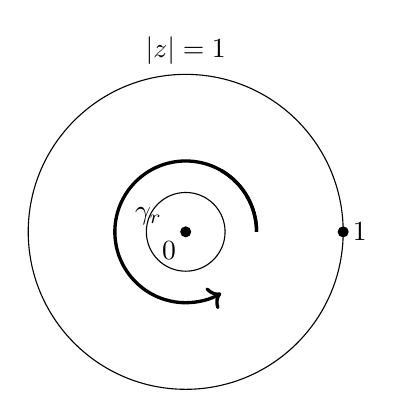
\begin{tikzpicture}[scale=2]
		% annulus boundaries
		\draw[thin] (0,0) circle (1);        % |z|=1
		\draw[thin] (0,0) circle (0.25);     % a small inner circle to suggest the hole
		% integration curve gamma_r
		\draw[very thick,->] (0.45,0) arc (0:300:0.45) node[pos=0.5,below right]{$\gamma_r$};
		\draw[very thick] (0.45,0) arc (0:60:0.45);
		% poles
		\fill (0,0) circle (1pt) node[below left]{$0$};
		\fill (1,0) circle (1pt) node[right]{$1$};
		\node at (0,1.15) {$|z|=1$};
	\end{tikzpicture}
	\caption{Part (a): $\gamma_r\subset\{0<|z|<1\}$ encloses $0$ but not $1$.}
\end{figure}

\begin{figure}[h]
	\centering
	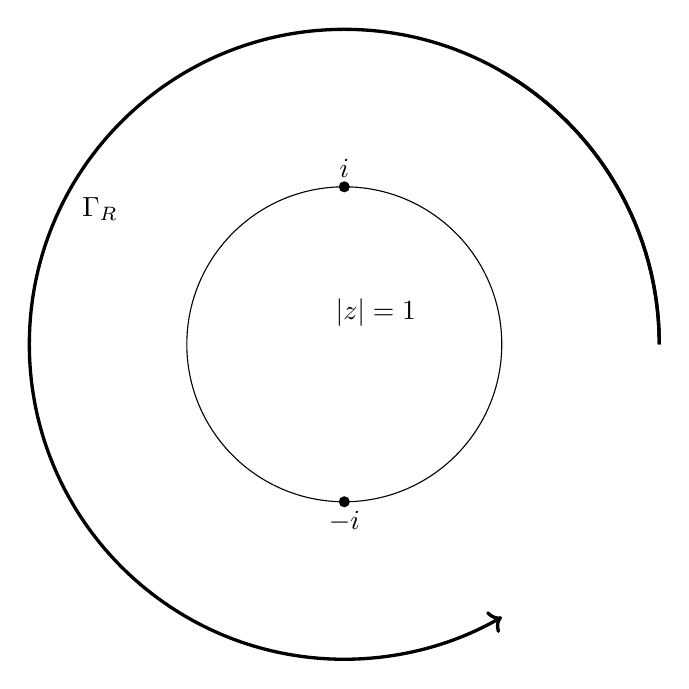
\begin{tikzpicture}[scale=2]
		% unit circle (hole) and big curve |z|=R
		\draw[thin] (0,0) circle (1);
		\draw[very thick,->] (2,0) arc (0:300:2) node[pos=0.5,below right]{$\Gamma_R$};
		\draw[very thick] (2,0) arc (0:60:2);
		% poles at ±i
		\fill (0,1) circle (1pt) node[above]{$i$};
		\fill (0,-1) circle (1pt) node[below]{$-i$};
		% labels
		\node at (0.2,0.2) {$|z|=1$};
	\end{tikzpicture}
	\caption{Part (b): $\Gamma_R\subset\{1<|z|<\infty\}$ encloses the poles $\pm i$.}
\end{figure}

\clearpage

\paragraph{Problem 11.}
Let $U\subset\mathbb C$ be a domain and $u:U\to\mathbb R$ be $C^2$ and harmonic.
Show that if $z_0\in U$, then for any disk $D=D(z_0,r)\Subset U$ there exists a holomorphic
$f:D\to\mathbb C$ with $\Re f=u$ on $D$.
Show by an example that this need not hold globally.

\medskip
\paragraph{Background.}
A $C^2$ real function $u$ is \emph{harmonic} if
\[
\Delta u \;=\; u_{xx}+u_{yy} \;=\; 0.
\]
Set the 1-form
\[
\alpha \;=\; -\,u_y\,dx \;+\; u_x\,dy.
\]
A short calculation gives
\[
d\alpha \;=\; (u_{xx}+u_{yy})\,dx\wedge dy \;=\; \Delta u\,dx\wedge dy.
\]
Hence if $u$ is harmonic, $\alpha$ is \emph{closed} ($d\alpha=0$).
On a simply connected domain (e.g.\ a disk), every closed 1-form is \emph{exact}, so there exists
$v$ with $dv=\alpha$, i.e.
\[
v_x=-u_y, \qquad v_y=u_x.
\]
Then the Cauchy–Riemann equations hold for $(u,v)$ and $f:=u+iv$ is holomorphic with $\Re f=u$.

\smallskip
On non–simply connected domains a closed form need not be exact; a certificate is a nonzero loop integral
\[
\oint_\gamma \alpha \;\neq\; 0
\qquad\text{for some closed curve }\gamma\subset U.
\]

\medskip
\paragraph{Solution.}

\emph{Local existence on a disk.}
Fix $z_0\in U$ and $D=D(z_0,r)\Subset U$.
Since $u$ is harmonic, $d\alpha=0$ on $D$. Because $D$ is simply connected,
there exists $v:D\to\mathbb R$ with $dv=\alpha$, i.e.
\[
v_x=-u_y, \qquad v_y=u_x.
\]
Hence the Cauchy–Riemann equations hold and
\[
f:=u+iv \quad\text{is holomorphic on } D \text{ with } \Re f=u.
\]

\medskip
\emph{Failure globally: a counterexample.}
Let $U=\mathbb C\setminus\{0\}$ and $u(z)=\log|z|$. Then $u\in C^\infty(U)$ and $\Delta u=0$.
If there were a holomorphic $F$ on $U$ with $\Re F=u$, then its imaginary part $v=\Im F$
would satisfy $dv=\alpha=-u_y\,dx+u_x\,dy$.

\smallskip
On the unit circle $\gamma(t)=e^{it}$, $0\le t\le 2\pi$, one has
\[
u_x=\frac{x}{x^2+y^2}, \qquad u_y=\frac{y}{x^2+y^2},
\]
so along $|z|=1$,
\[
\oint_{\gamma}\alpha
=\oint_{\gamma}(-y\,dx+x\,dy)
=\int_0^{2\pi}\!\!\big(-\sin t\cdot(-\sin t)+\cos t\cdot\cos t\big)\,dt
=\int_0^{2\pi}\!1\,dt
=2\pi \;\neq\; 0.
\]
Thus $\alpha$ is not exact on $U$, so no global $v$ exists and $u$ is \emph{not}
the real part of any holomorphic function on $U$.
\qed

\paragraph{Problem 1.}
\begin{enumerate}[label=(\roman*)]
	\item Use Cauchy’s integral formula to compute
	\[
	\int_{|z|=1}\frac{e^{\alpha z}}{2z^{2}-5z+2}\,dz,\qquad \alpha\in\mathbb C.
	\]
	
	\item By considering the real part of a suitable complex integral, show that for $r\in(0,1)$,
	\[
	\int_{0}^{\pi}\frac{\cos(n\theta)}{1-2r\cos\theta+r^{2}}\,d\theta=\frac{\pi r^{n}}{1-r^{2}},
	\qquad
	\int_{0}^{2\pi}\cos(\cos\theta)\cosh(\sin\theta)\,d\theta=2\pi .
	\]
\end{enumerate}

\paragraph{Background.}
Cauchy’s integral formula: if $f$ is holomorphic on and inside a simple closed curve $\gamma$, then
$\displaystyle \int_\gamma \frac{f(z)}{z-a}\,dz=2\pi i\,f(a)$ for $a$ inside $\gamma$.
Also, with $z=e^{i\theta}$ one has $d\theta=\frac{dz}{iz}$ and
$1-2r\cos\theta+r^{2}=(1-rz)(1-rz^{-1})=\frac{(z-r)(1-rz)}{z}$.

\paragraph{Solution.}
\emph{(i)} Factor $2z^{2}-5z+2=2(z-2)\bigl(z-\tfrac12\bigr)$. On $|z|=1$ only $z=\tfrac12$ lies inside.
Hence
\[
\int_{|z|=1}\frac{e^{\alpha z}}{2z^{2}-5z+2}\,dz
=2\pi i\cdot \Res\!\left(\frac{e^{\alpha z}}{2(z-2)\bigl(z-\tfrac12\bigr)};\ \tfrac12\right)
=2\pi i\cdot \frac{e^{\alpha/2}}{2(\tfrac12-2)}
=-\,\frac{2\pi i}{3}\,e^{\alpha/2}.
\]

\medskip
\emph{(ii-a)} Let
\[
I_n=\int_{0}^{2\pi}\frac{e^{in\theta}}{1-2r\cos\theta+r^{2}}\,d\theta.
\]
With $z=e^{i\theta}$ and $d\theta=\frac{dz}{iz}$,
\[
I_n=\oint_{|z|=1}\frac{z^{n}}{(z-r)(1-rz)}\,\frac{dz}{i}.
\]
Only $z=r$ lies inside, giving $\Res=\dfrac{r^{n}}{1-r^{2}}$. Thus
\[
I_n=2\pi\,\frac{r^{n}}{1-r^{2}},\qquad
\int_{0}^{2\pi}\frac{\cos(n\theta)}{1-2r\cos\theta+r^{2}}\,d\theta
=\Re I_n=\frac{2\pi r^{n}}{1-r^{2}}.
\]
Halving the interval,
\[
\int_{0}^{\pi}\frac{\cos(n\theta)}{1-2r\cos\theta+r^{2}}\,d\theta
=\frac{\pi r^{n}}{1-r^{2}}.
\]

\medskip
\emph{(ii-b)} Using
$\cos(\cos\theta)\cosh(\sin\theta)=\tfrac12\big(e^{i e^{i\theta}}+e^{-i e^{i\theta}}\big)$,
\[
\int_{0}^{2\pi}\cos(\cos\theta)\cosh(\sin\theta)\,d\theta
=\frac12\oint_{|z|=1}\frac{e^{iz}+e^{-iz}}{iz}\,dz
=\frac{1}{2i}\cdot 2\pi i\,\bigl(e^{0}+e^{0}\bigr)=2\pi.
\]
\qed


% In the preamble (once):
% \usepackage{amsmath,amssymb,amsthm}
% \DeclareMathOperator{\Res}{Res}

\paragraph{Residues: definitions, equivalences, and tools.}

\medskip
\emph{Laurent series and the residue.}
Let $f$ be meromorphic with an isolated singularity at $a$.
Then there is $\rho>0$ and integers $m\ge 0$ and coefficients $\{c_k\}_{k=-m}^{\infty}$ such that
\[
f(z)=\sum_{k=-m}^{\infty} c_k (z-a)^k, \qquad 0<|z-a|<\rho .
\]
\textbf{Definition.} The \emph{residue} of $f$ at $a$ is the coefficient of $(z-a)^{-1}$:
\[
\boxed{\ \Res(f;a)=c_{-1}\ }.
\]

\medskip
\emph{Equivalent characterizations.}
For any $0<\varepsilon<\rho$,
\[
\Res(f;a)=\frac{1}{2\pi i}\oint_{|z-a|=\varepsilon} f(z)\,dz.
\]
If $a$ is a simple pole (i.e.\ $m=1$), then
\[
\Res(f;a)=\lim_{z\to a} (z-a)\,f(z).
\]
More generally, if $a$ is a pole of order $m$,
\[
\Res(f;a)=\frac{1}{(m-1)!}\lim_{z\to a}\frac{d^{\,m-1}}{dz^{m-1}}\big((z-a)^m f(z)\big).
\]

\smallskip
\emph{Proof sketch of $c_{-1}$-rule.}
Write the Laurent series and integrate termwise on $|z-a|=\varepsilon$:
\[
\oint (z-a)^k\,dz = \begin{cases}
	0, & k\neq -1,\\[2pt]
	2\pi i, & k=-1.
\end{cases}
\]
Thus $\displaystyle \oint f = 2\pi i\,c_{-1}$ and $\Res(f;a)=c_{-1}$.

\medskip
\emph{Residue Theorem (workhorse).}
If $f$ is meromorphic on and inside a positively oriented simple closed curve $\gamma$
with no poles on $\gamma$, then
\[
\int_{\gamma} f(z)\,dz
= 2\pi i \sum_{a_k\in \mathrm{Int}(\gamma)} \Res(f;a_k).
\]

\medskip
\emph{Quick computation rules.}
\begin{itemize}
	\item \textbf{Simple pole formula.} If $f(z)=\dfrac{p(z)}{q(z)}$ with $p,q$ holomorphic,
	$q(a)=0$, $q'(a)\neq 0$, then
	\[
	\Res(f;a)=\frac{p(a)}{q'(a)}.
	\]
	\item \textbf{Analytic factor.} If $g$ is holomorphic near $a$, then
	$\Res(g\,f;a)=g(a)\,\Res(f;a)$.
	\item \textbf{Pole at infinity.} If $f$ is meromorphic on the Riemann sphere $\widehat{\mathbb C}$,
	\[
	\Res(f;\infty) := -\sum_{a\in\mathbb C}\Res(f;a),\qquad
	\oint_{|z|=R} f(z)\,dz \xrightarrow{R\to\infty} -2\pi i\,\Res(f;\infty),
	\]
	when the outer integral stabilizes.
\end{itemize}

\medskip
\emph{Micro–examples (via $c_{-1}$).}
\begin{itemize}
	\item $f(z)=\dfrac{1}{(z-a)(z-b)}$ near $a$: expand
	\(
	\dfrac{1}{z-b}=\dfrac{1}{a-b} + O(z-a)
	\),
	so
	\[
	f(z)=\frac{1}{z-a}\cdot \frac{1}{a-b} + O(1)
	\;\Rightarrow\;
	\Res(f;a)=\frac{1}{a-b}.
	\]
	\item $f(z)=\dfrac{e^{\alpha z}}{(z-a)(z-b)}$ near $a$:
	\(
	e^{\alpha z}=e^{\alpha a}+O(z-a)
	\), hence
	\[
	f(z)=\frac{1}{z-a}\cdot \frac{e^{\alpha a}}{a-b}+O(1)
	\;\Rightarrow\;
	\Res(f;a)=\frac{e^{\alpha a}}{a-b}.
	\]
\end{itemize}

\medskip
\emph{Unit-circle substitution for trig integrals.}
With $z=e^{i\theta}$, $d\theta=\dfrac{dz}{iz}$ and
\[
1-2r\cos\theta+r^2=(1-rz)(1-rz^{-1})=\frac{(z-r)(1-rz)}{z}.
\]
Only $z=r$ lies inside $|z|=1$ if $0<r<1$, giving
\[
\int_{0}^{2\pi}\frac{e^{in\theta}}{1-2r\cos\theta+r^2}\,d\theta
=\oint_{|z|=1}\frac{z^n}{(z-r)(1-rz)}\,\frac{dz}{i}
=2\pi\,\frac{r^n}{1-r^2}.
\]
Taking real parts yields
\(
\displaystyle \int_{0}^{\pi}\frac{\cos(n\theta)}{1-2r\cos\theta+r^2}\,d\theta=\frac{\pi r^n}{1-r^2}.
\)

\paragraph{Problem 2.}
Find the Laurent expansion (in powers of $z$, i.e.\ about $0$) of
\[
\frac{1}{z^{2}-3z+2}=\frac{1}{(z-1)(z-2)}
\]
in the regions $\{|z|<1\}$, $\{1<|z|<2\}$, and $\{|z|\ge 2\}$.

\paragraph{Background.}
Partial fractions:
\[
\frac{1}{(z-1)(z-2)}=-\frac{1}{z-1}+\frac{1}{z-2}.
\]
Geometric expansions:
\[
\frac{1}{1-w}=\sum_{n=0}^{\infty}w^{n}\quad(|w|<1),\qquad
\frac{1}{z-a}=\frac{1}{z}\cdot\frac{1}{1-\frac{a}{z}}
=\sum_{n=0}^{\infty}\frac{a^{n}}{z^{n+1}}\quad(|z|>|a|).
\]

\paragraph{Solutions.}

\emph{(A) For $|z|<1$.}
\[
-\frac{1}{z-1}=\frac{1}{1-z}=\sum_{n=0}^{\infty}z^{n},\qquad
\frac{1}{z-2}=-\frac{1}{2}\frac{1}{1-\frac{z}{2}}
=-\sum_{n=0}^{\infty}\frac{z^{n}}{2^{\,n+1}}.
\]
Hence
\[
\boxed{\ \frac{1}{z^{2}-3z+2}=\sum_{n=0}^{\infty}\Big(1-2^{-(n+1)}\Big)z^{n},\quad |z|<1.\ }
\]

\medskip
\emph{(B) For $1<|z|<2$.}
\[
-\frac{1}{z-1}=-\frac{1}{z}\frac{1}{1-\frac{1}{z}}
=-\sum_{n=1}^{\infty} z^{-n},\qquad
\frac{1}{z-2}=-\sum_{n=0}^{\infty}\frac{z^{n}}{2^{\,n+1}}.
\]
Thus
\[
\boxed{\ \frac{1}{z^{2}-3z+2}
	=-\sum_{n=1}^{\infty} z^{-n}-\sum_{n=0}^{\infty}\frac{z^{n}}{2^{\,n+1}},
	\quad 1<|z|<2.\ }
\]

\medskip
\emph{(C) For $|z|>2$.}
\[
-\frac{1}{z-1}=-\sum_{m=1}^{\infty} z^{-m},\qquad
\frac{1}{z-2}=\frac{1}{z}\frac{1}{1-\frac{2}{z}}
=\sum_{m=1}^{\infty}\frac{2^{\,m-1}}{z^{m}}.
\]
Therefore
\[
\boxed{\ \frac{1}{z^{2}-3z+2}
	=\sum_{m=1}^{\infty}\big(2^{\,m-1}-1\big)z^{-m},\quad |z|>2.\ }
\]
\qed

\paragraph{Problem 3.}
Classify the singularities of
\[
\frac{z}{\sin z},\qquad
\sin\!\Big(\frac{\pi}{z^{2}}\Big),\qquad
\frac{1}{z^{2}}+\frac{1}{z^{2}+1},\qquad
\frac{1}{z^{2}}\cos\!\Big(\frac{\pi z}{z+1}\Big).
\]

\paragraph{Background.}
At an isolated singularity $a$, if the Laurent expansion
$f(z)=\sum_{k=-m}^{\infty} c_k (z-a)^k$ has
(i) $m=0$ $\Rightarrow$ removable;
(ii) finitely many negative terms with highest $(z-a)^{-m}$ $\Rightarrow$ pole of order $m$;
(iii) infinitely many negative terms $\Rightarrow$ essential.

\medskip
\emph{(1) $\boldsymbol{z/\sin z}$.}
Near $0$, $\sin z=z-\frac{z^{3}}{6}+O(z^{5})$, so
\[
\frac{z}{\sin z}=1+\frac{z^{2}}{6}+O(z^{4}),
\]
hence $z=0$ is \textbf{removable} (define value $1$). At $z=n\pi$, $n\in\mathbb Z\setminus\{0\}$,
$\sin z$ has simple zeros and the numerator is nonzero, so each $n\pi$ is a \textbf{simple pole}.

\medskip
\emph{(2) $\boldsymbol{\sin(\pi/z^{2})}$.}
Using $\sin w=\sum_{k\ge0}\frac{(-1)^k w^{2k+1}}{(2k+1)!}$ with $w=\pi/z^{2}$,
\[
\sin\!\Big(\frac{\pi}{z^{2}}\Big)=\sum_{k=0}^{\infty}\frac{(-1)^k \pi^{2k+1}}{(2k+1)!}\,z^{-4k-2},
\]
which contains infinitely many negative powers. Thus $z=0$ is an \textbf{essential singularity}.
There are no other singularities.

\medskip
\emph{(3) $\boldsymbol{1/z^{2} + 1/(z^{2}+1)}$.}
At $z=0$ one has a \textbf{pole of order $2$}. At $z=\pm i$ (simple zeros of $z^{2}+1$) there are
\textbf{simple poles}. No other singularities occur.

\medskip
\emph{(4) $\boldsymbol{z^{-2}\cos\!\big(\pi z/(z+1)\big)}$.}
Let $h(z)=\dfrac{\pi z}{z+1}$.
Near $z=0$, $h(z)=\pi(z-z^{2}+z^{3}-\cdots)$, hence
\[
\cos h(z)=1-\tfrac12 h(z)^{2}+O(z^{3})=1-\tfrac{\pi^{2}}{2}z^{2}+O(z^{3}),
\]
and
\[
\frac{1}{z^{2}}\cos h(z)=\frac{1}{z^{2}}-\frac{\pi^{2}}{2}+O(z),
\]
so $z=0$ is a \textbf{pole of order $2$}. At $z=-1$, $h$ has a simple pole; since
$\cos w=\tfrac12(e^{iw}+e^{-iw})$, composition with a pole yields an \textbf{essential singularity}
at $z=-1$. There are no other singularities.
\qed

\paragraph{Problem 4.}
Let $f:\mathbb C\to\mathbb C$ be entire. Prove that $f$ is constant if any one of the following holds:
\begin{enumerate}[label=(\roman*)]
	\item $\displaystyle \frac{f(z)}{z}\to 0$ as $|z|\to\infty$.
	\item There exist $b\in\mathbb C$ and $\varepsilon>0$ such that $|f(z)-b|>\varepsilon$ for all $z\in\mathbb C$.
	\item Writing $f=u+iv$ with real $u,v$, one has $|u(z)|>|v(z)|$ for all $z\in\mathbb C$.
\end{enumerate}

\paragraph{Background.}
We use: (a) \emph{Liouville’s theorem}: a bounded entire function is constant; (b) \emph{Cauchy estimates}:
if $f$ is holomorphic on $|z|\le R$, then $|f^{(n)}(0)|\le \dfrac{n!}{R^n}\max_{|z|=R}|f(z)|$; 
(c) the Cayley map $w\mapsto \dfrac{w-1}{w+1}$ sends $\{\Re w>0\}$ to the unit disk; 
(d) if $FG\equiv 0$ with $F,G$ holomorphic on a connected set, then $F\equiv 0$ or $G\equiv 0$.

\paragraph{Solution.}

\emph{(i) Sublinear growth.}
Given $\eta>0$, choose $R_\eta$ so that $|f(z)|\le \eta|z|$ for $|z|\ge R_\eta$.
For $R\ge R_\eta$,
\[
\max_{|z|=R}|f(z)|\le \eta R.
\]
Cauchy estimates at $0$ yield
\[
|f^{(n)}(0)|\le \frac{n!\,\eta R}{R^n}=\frac{n!\,\eta}{R^{n-1}}\quad(n\ge 1).
\]
Letting $R\to\infty$ gives $f^{(n)}(0)=0$ for $n\ge 2$, and $|f'(0)|\le \eta$ for all $\eta>0$, hence $f'(0)=0$.
Thus $f$ is constant.

\medskip
\emph{(ii) Image avoids a disk.}
If $|f(z)-b|>\varepsilon$ for all $z$, then $g(z)=\dfrac{1}{f(z)-b}$ is entire and bounded by $1/\varepsilon$.
By Liouville, $g$ is constant, hence $f$ is constant.

\medskip
\emph{(iii) Real part dominates.}
If $f=u+iv$ with $|u|>|v|$ everywhere, then $\Re\big(f^2\big)=u^2-v^2>0$, so $g:=f^2$ maps $\mathbb C$ into the right half–plane.
The Cayley transform $h=(g-1)/(g+1)$ is entire and satisfies $|h|<1$, hence $h$ is constant by Liouville, so $g\equiv c$ with $\Re c>0$.
Therefore $(f-\sqrt c)(f+\sqrt c)\equiv 0$, and by analyticity one factor vanishes identically.
Thus $f\equiv \sqrt c$ or $f\equiv -\sqrt c$, i.e. $f$ is constant.
\qed

\paragraph{Problem 6.}
\begin{enumerate}[label=(\roman*)]
	\item Let $f$ be entire. Show that $f$ is a polynomial of degree $\le k$ iff there is $M>0$ with
	\[
	|f(z)|\le M(1+|z|)^k\qquad(\forall z\in\mathbb C).
	\]
	\item Show that an entire $f$ is a polynomial of positive degree iff $|f(z)|\to\infty$ as $|z|\to\infty$.
	\item Let $f$ be analytic on $\mathbb C$ apart from finitely many poles. If there exists $k$ such that
	$|f(z)|\le |z|^k$ for all sufficiently large $|z|$, prove that $f$ is a rational function.
\end{enumerate}

\paragraph{Background.}
\emph{Cauchy estimates.} If $f$ is holomorphic on $|z|\le R$, then
\[
|f^{(n)}(0)|\le \frac{n!}{R^n}\max_{|z|=R}|f(z)|.
\]
\emph{Poles at infinity.} For $g(w)=f(1/w)$ near $w=0$, a pole of order $m$ at $0$ means $f$ has a pole at $\infty$ of order $m$. An entire function with a pole at $\infty$ is a polynomial (degree $m$). A function meromorphic on the Riemann sphere (only poles, finitely many) is rational.

\paragraph{Solution.}
\emph{(i) $\Leftarrow$.}
Assume $|f(z)|\le M(1+|z|)^k$. For $R>0$, $\max_{|z|=R}|f(z)|\le M(1+R)^k$. Hence
\[
|f^{(n)}(0)|\le \frac{n!}{R^n}M(1+R)^k \qquad (n\ge 0).
\]
Fix $n>k$ and let $R\to\infty$: $(1+R)^k/R^n\to 0$, so $f^{(n)}(0)=0$. Therefore the Taylor series truncates at degree $\le k$ and $f$ is a polynomial.

\smallskip
\emph{(i) $\Rightarrow$.}
If $f(z)=\sum_{j=0}^k a_j z^j$, then $|f(z)|\le \sum_{j=0}^k |a_j||z|^j \le C(1+|z|)^k$.

\medskip
\emph{(ii) $\Rightarrow$.}
If $f$ is a nonconstant polynomial of degree $m\ge 1$, then $|f(z)|\sim |a_m||z|^m\to\infty$.

\emph{(ii) $\Leftarrow$.}
If $|f(z)|\to\infty$ as $|z|\to\infty$, then $g(w)=f(1/w)$ has a pole at $w=0$, so $f$ has a pole at $\infty$ and is therefore a polynomial of positive degree.

\medskip
\emph{(iii).}
Let $g(w)=f(1/w)$. For small $|w|$,
\[
|g(w)|=|f(1/w)|\le |1/w|^k=|w|^{-k},
\]
so $g$ has at most a pole of order $\le k$ at $0$. Hence $f$ has at most a pole at $\infty$. Together with the finitely many poles in $\mathbb C$, $f$ is meromorphic on the Riemann sphere with only poles; thus $f$ is rational.
\qed

\paragraph{Problem 7.}
\begin{enumerate}[label=(\roman*)]
	\item (\textbf{Schwarz's Lemma}) Let $f$ be analytic on $D(0,1)$ with $|f(z)|\le 1$ and $f(0)=0$.
	Apply the maximum principle to $f(z)/z$ to show $|f(z)|\le |z|$. Show also that if $|f(w)|=|w|$ for some $w\neq 0$, then $f(z)=c\,z$ for some constant $c$.
	
	\item Use Schwarz's Lemma to prove that any conformal equivalence $\Phi:D(0,1)\to D(0,1)$ is given by a Möbius transformation.
\end{enumerate}

\paragraph{Background.}
If a holomorphic $g$ on $0<|z|<1$ is bounded near $0$, then $g$ extends holomorphically to $z=0$ (removable singularity).
A non-constant holomorphic function does not attain a maximum of its modulus in the interior (maximum modulus principle).
For $a\in D$, the map $\displaystyle \phi_a(z)=\frac{z-a}{1-\overline a\,z}$ is a biholomorphism $D\to D$ with $\phi_a(a)=0$.

\paragraph{Solution.}

\emph{(i)} Define
\[
g(z)=\begin{cases}
	\dfrac{f(z)}{z},& z\neq 0,\\[4pt]
	f'(0),& z=0.
\end{cases}
\]
Because $|f(z)|\le 1$ and $f(0)=0$, $g$ is bounded near $0$, hence extends holomorphically to $D$.
For $0<r<1$, on $|z|=r$ we have $|g(z)|\le 1/r$. By the maximum modulus principle on each smaller disk, letting $r\uparrow 1$ gives $|g(z)|\le 1$ for all $z\in D$.
Thus $|f(z)|\le |z|$ and $|f'(0)|=|g(0)|\le 1$.

If $|f(w)|=|w|$ for some $w\ne 0$, then $|g(w)|=1$. By the maximum modulus principle $g$ has constant modulus $1$ on $D$, hence $g\equiv c$ with $|c|=1$ and $f(z)=c\,z$.

\medskip
\emph{(ii)} Let $\Phi:D\to D$ be a conformal bijection and set $a=\Phi(0)$. Consider $F=\phi_a\circ \Phi$, where $\displaystyle \phi_a(z)=\frac{z-a}{1-\overline a\,z}$.
Then $F:D\to D$ is holomorphic with $F(0)=0$. By Schwarz's Lemma, $F(z)=\lambda z$ with $|\lambda|\le 1$; since $\Phi$ is bijective, $| \lambda|=1$.
Therefore
\[
\Phi(z)=\phi_a^{-1}(\lambda z)=\lambda\,\frac{z-a}{1-\overline a\,z},
\]
a Möbius automorphism of the disk.
\qed

\paragraph{Conformal maps and conformal equivalence.}

\emph{Conformal at a point.}
A map $f:U\to\mathbb C$ is conformal at $z_0\in U$ if it preserves angles between smooth curves through $z_0$ (with orientation). In complex analysis this is equivalent to
\[
f \text{ holomorphic at } z_0 \quad\text{and}\quad f'(z_0)\neq 0.
\]
Indeed, the first-order expansion $f(z)=f(z_0)+f'(z_0)(z-z_0)+o(|z-z_0|)$ shows $f$ is locally “rotation $+\,$dilation”. Writing $f=u+iv$, the Cauchy--Riemann equations at $z_0$ give
\[
Df(z_0)=
\begin{pmatrix}u_x & u_y\\ v_x & v_y\end{pmatrix}
=
\begin{pmatrix}a & -b\\ b & a\end{pmatrix}
=|f'(z_0)|
\begin{pmatrix}\cos\theta & -\sin\theta\\ \sin\theta & \cos\theta\end{pmatrix},
\]
so $Df(z_0)$ is a positive scalar times a rotation, hence angle-preserving and orientation-preserving.

\emph{Angle preservation formula.}
If $v_1,v_2\in\mathbb C$ are tangent directions at $z_0$, then under $f$
\[
\cos\angle(f_*v_1,f_*v_2)
=\frac{\Re\big((f'(z_0)v_1)\overline{(f'(z_0)v_2)}\big)}{|f'(z_0)v_1|\,|f'(z_0)v_2|}
=\frac{\Re(v_1\overline{v_2})}{|v_1||v_2|},
\]
so the angle is unchanged.

\emph{Conformal equivalence.}
Domains $U,V\subset\mathbb C$ are \emph{conformally equivalent} if there is a biholomorphism $f:U\to V$ (holomorphic and bijective with holomorphic inverse). Such an $f$ is conformal on $U$, and $f^{-1}$ is conformal on $V$.

\emph{Examples.}
\begin{itemize}
	\item Cayley transform $\displaystyle \phi(z)=\frac{z-i}{\,z+i\,}$: biholomorphism $\{\Im z>0\}\leftrightarrow\mathbb D$.
	\item Exponential $\displaystyle w=e^{\pi z}$: biholomorphism $\,\{0<\Im z<1\}\leftrightarrow \{1<|w|<e^{\pi}\}$.
\end{itemize}

\emph{Non-examples.}
\begin{itemize}
	\item $f(z)=z^n$ is not conformal at $z=0$ for $n\ge 2$ since $f'(0)=0$ (angles multiply by $n$).
	\item Conjugation $f(z)=\overline z$ reverses orientation (anti-conformal).
\end{itemize}

% ---------- Problem 8 (statement) ----------
\paragraph{Problem 8 (restated).}
\begin{enumerate}[label=(\roman*)]
	\item Let $f$ be entire and satisfy $f(1/n)=1/n$ for all $n\in\mathbb N$. Prove that $f(z)\equiv z$.
	\item Let $f$ be entire and satisfy $f(n)=n^{2}$ for all $n\in\mathbb Z$. Must $f$ equal $z^{2}$? Give a justification or a counterexample.
	\item Let $f$ be holomorphic on $D(0,2)$. Show that there exists $n\in\mathbb N$ with $f(1/n)\ne 1/(n+1)$.
\end{enumerate}

\medskip
% ---------- Background for Problem 8 ----------
\paragraph{Background and definitions for Problem 8.}

\emph{Holomorphic / entire.}
A function $f$ is holomorphic on a domain $U\subset\mathbb C$ if it is complex differentiable at every point of $U$.
It is \emph{entire} if it is holomorphic on all of $\mathbb C$.
A \emph{domain} is a nonempty, open, connected subset of $\mathbb C$.

\medskip
\emph{Accumulation point.}
A sequence $(z_n)\subset U$ has an accumulation point $z_\ast\in U$ if $z_n\to z_\ast$ with $z_n\neq z_\ast$ eventually.

\medskip
\emph{Isolated zeros and the identity theorem.}
If $f$ is holomorphic on $U$ and not identically zero, then its zeros have no accumulation point in $U$.
If $f,g$ are holomorphic on $U$ and $f=g$ on a set with a limit point in $U$ (e.g.\ $z_n\to z_\ast\in U$), then $f\equiv g$ on $U$.
Equivalently, if a holomorphic $f$ vanishes on such a set, then $f\equiv 0$.

\medskip
\emph{An entire function vanishing on $\mathbb Z$.}
$\sin(\pi z)$ is entire and $\sin(\pi n)=0$ for all $n\in\mathbb Z$.
Thus for prescribed integer values, one may add $\sin(\pi z)\cdot H(z)$ (with $H$ entire) without changing those values.

\medskip
\emph{Removable singularities (Riemann).}
If $f$ is holomorphic on $0<|z-a|<r$ and bounded near $a$, then $f$ extends holomorphically to $z=a$.

\medskip
\emph{How these tools are used in Problem 8.}
\begin{itemize}
	\item \textbf{(i)} $g(z)=f(z)-z$ entire with $g(1/n)=0$ and $1/n\to 0\in\mathbb C$ $\Rightarrow$ $g\equiv 0$.
	\item \textbf{(ii)} Integers have no accumulation in $\mathbb C$; non-uniqueness via $\sin(\pi z)$.
	\item \textbf{(iii)} Zeros at $1/n\to 0$ in $D(0,2)\setminus\{-1\}$ force identity with a meromorphic function that has a pole at $-1$ — contradiction.
\end{itemize}

\medskip
% ---------- Problem 8 (solution) ----------
\paragraph{Solution to Problem 8.}

\begin{enumerate}[label=(\roman*)]
	\item Define
	\[
	g(z):=f(z)-z .
	\]
	Then $g$ is entire and $g(1/n)=0$ for all $n$. Since $1/n\to 0$ (an interior point),
	the identity theorem gives $g\equiv 0$, hence $f(z)\equiv z$.
	
	\medskip
	\item Not necessarily. For example,
	\[
	f(z)=z^{2}+\sin(\pi z)
	\]
	is entire and satisfies $f(n)=n^{2}$ for all $n\in\mathbb Z$, yet $f\not\equiv z^{2}$.
	
	\medskip
	\item Suppose $f(1/n)=1/(n+1)$ for all $n$. Then
	\[
	h(z):=f(z)-\frac{z}{z+1}
	\]
	is holomorphic on $D(0,2)\setminus\{-1\}$, vanishes at $z=1/n$ for all $n$, and the set $\{1/n\}$ accumulates at $0$ in that domain.
	By the identity theorem, $h\equiv 0$ there, i.e.\ $f(z)=\dfrac{z}{z+1}$ on $D(0,2)\setminus\{-1\}$.
	But $\dfrac{z}{z+1}$ has a pole at $z=-1$, whereas $f$ is holomorphic there — a contradiction.
	Hence some $n$ satisfies $f(1/n)\ne 1/(n+1)$.
\end{enumerate}

\bigskip
% ---------- Problem 9 (statement) ----------
\paragraph{Problem 9 (Casorati--Weierstrass; restated).}
If $f$ is holomorphic on $D(a,R)\setminus\{a\}$ with an essential singularity at $a$, then for any $b\in\mathbb C$
there exists a sequence $z_n\to a$ such that $f(z_n)\to b$.

\medskip
\paragraph{Solution to Problem 9.}
If $f$ omitted $b$ near $a$, then $g=1/(f-b)$ would be bounded near $a$, hence removable there by Riemann’s theorem.
Thus $f=b+1/g$ would have at worst a pole/removable singularity at $a$, contradicting essentiality.
\emph{Example.} For $f(z)=e^{1/z}$, $a=0$, $b=2$, take
\[
z_n=\frac{1}{\Log 2+2\pi i n}\quad\Rightarrow\quad e^{1/z_n}=2 .
\]

\bigskip
% ---------- Problem 10 (statement) ----------
\paragraph{Problem 10 (restated).}
Let $D\subset\mathbb C$ be simply connected and $0\notin D$.
Show that there exists a holomorphic function $F$ on $D$ with $F'(z)=1/z$ and $e^{F(z)}=z$ for $z\in D$
(i.e.\ $F$ is a branch of the logarithm on $D$).

\medskip
\paragraph{Solution to Problem 10.}
Fix $z_0\in D$ and define
\[
F(z)=\int_{z_0}^{z}\frac{d\zeta}{\zeta}.
\]
Since $1/\zeta$ is holomorphic on $D$ and $D$ is simply connected, the integral is path-independent; $F$ is holomorphic with $F'(z)=1/z$.
Let $G(z)=e^{F(z)}/z$. Then $G'(z)=0$, so $G$ is constant. Choosing $F(z_0)$ so that $G\equiv 1$ yields $e^{F(z)}=z$ on $D$.

\bigskip
% ---------- Problem 11 (statement) ----------
\paragraph{Problem 11 (restated).}
Consider the lacunary series
\[
f(z)=\sum_{n=1}^{\infty} z^{2^{n}} .
\]
Show that it defines an analytic function on $D(0,1)$ but admits no analytic continuation across any point of $|z|=1$.

\medskip
\paragraph{Solution to Problem 11.}
The series converges absolutely and uniformly on compact subsets of $D(0,1)$, so $f$ is analytic there.
Moreover, for $m\ge 1$,
\[
(1-z^{2^{m}})f(z)=\sum_{j=1}^{m-1} z^{2^{j}},
\]
so each $2^{m}$-th root of unity is a singularity of $f$ (unless trivially canceled).
As the union $\bigcup_{m\ge 1}\{\zeta:\zeta^{2^{m}}=1\}$ is dense on $|z|=1$, $|z|=1$ is a \emph{natural boundary}:
no analytic continuation is possible across any boundary point.
% (Alternatively, cite the Hadamard gap theorem since $2^{n+1}/2^{n}=2$.)
\qed


\paragraph{Background for Problems 9--11.}

\emph{Domains and basic classes.}
A \emph{domain} is a nonempty, open, connected subset of $\mathbb C$.
A function is \emph{holomorphic} on $U$ if it is complex differentiable at every point of $U$.
It is \emph{entire} if holomorphic on $\mathbb C$.
It is \emph{meromorphic} on $U$ if holomorphic on $U$ except at isolated poles.

\medskip
\emph{Isolated singularities.}
Let $f$ be holomorphic on $0<|z-a|<r$. Then $a$ is an \emph{isolated singularity} and exactly one holds:
\begin{itemize}
	\item \textbf{Removable:} $f$ is bounded near $a$ $\Rightarrow$ $f$ extends holomorphically to $a$ (Riemann).
	\item \textbf{Pole:} $|f(z)|\to\infty$ as $z\to a$; equivalently, $(z-a)^m f(z)$ extends holomorphically with nonzero value at $a$ for some $m\in\mathbb N$.
	\item \textbf{Essential:} neither removable nor pole. The Laurent expansion at $a$ then has infinitely many negative powers.
\end{itemize}

\medskip
\emph{Casorati--Weierstrass \& Picard (context for Problem 9).}
If $a$ is an essential singularity of $f$, then the image of any punctured neighborhood of $a$ is dense in $\mathbb C$
(Casorati--Weierstrass). A stronger statement (Great Picard) says that near an essential singularity $f$ attains every complex value, with at most one exception, infinitely often.

\medskip
\emph{Identity theorem \& isolated zeros.}
If $f,g$ are holomorphic on a domain $U$ and $f=g$ on a set with a limit point in $U$, then $f\equiv g$ on $U$.
Consequently, a nonzero holomorphic function on $U$ has zeros that do not accumulate in $U$.

\medskip
\emph{Path independence and primitives (for Problem 10).}
If $\omega(z)\,dz$ is holomorphic on a simply connected domain $D$, then
\[
F(z):=\int_{z_0}^{z}\omega(\zeta)\,d\zeta
\]
is well defined (independent of path), holomorphic on $D$, and satisfies $F'=\omega$.
In particular, if $0\notin D$, the $1$-form $d\zeta/\zeta$ has the primitive
$F(z)=\int_{z_0}^z \frac{d\zeta}{\zeta}$ on $D$, so $e^{F}$ gives a single-valued branch of the logarithm.

\smallskip
\emph{Winding number criterion for a logarithm.}
A holomorphic, nowhere–vanishing function $g$ on a domain $D$ admits a holomorphic branch of $\Log g$ on $D$
iff $\displaystyle \int_{\gamma} \frac{g'}{g}\,dz=0$ for every closed curve $\gamma\subset D$;
equivalently, $g(\gamma)$ has winding number $0$ about $0$ for all such $\gamma$.
When $D$ is simply connected and $g$ never vanishes, a branch of $\Log g$ always exists.

\medskip
\emph{Power series, radius of convergence, and natural boundaries (for Problem 11).}
A power series $\sum_{n\ge0} a_n z^n$ has a radius of convergence $R\in[0,\infty]$ determined by the Cauchy--Hadamard formula.
It defines an analytic function on $|z|<R$ and cannot be analytically continued across points where the function has a singularity.
A Jordan curve $\Gamma$ is a \emph{natural boundary} for $f$ if no analytic continuation of $f$ exists across \emph{any} point of $\Gamma$.

\smallskip
\emph{Hadamard gap theorem (lacunary series).}
If $f(z)=\sum_{k\ge1} a_k z^{n_k}$ with strictly increasing exponents $(n_k)$ satisfying
$\displaystyle \liminf_{k\to\infty} \frac{n_{k+1}}{n_k}>1$ (``Hadamard gaps''),
then the circle of convergence $|z|=R$ is a \emph{natural boundary} for $f$ (unless $f$ is a polynomial).
In particular, for $n_k=2^k$ (ratio $=2$) the unit circle is a natural boundary when $R=1$.

\medskip
\emph{Dense boundary singularities via functional identities (alternate route for Problem 11).}
If a function $f$ on $|z|<1$ satisfies identities of the form
\[
(1-z^{N})\,f(z)=P_N(z)\qquad (N\in\mathbb N),
\]
with $P_N$ polynomial and $N\to\infty$, then every $N$-th root of unity
is a singularity (unless canceled), and the union of these roots for $N\to\infty$ is dense on $|z|=1$.
Hence $|z|=1$ is a natural boundary (no analytic continuation across any boundary point).

\paragraph{Problem.}
Let $f$ be holomorphic on $D(a,R)$. If $w$ satisfies $|w-a|<r<R$, show
\[
f^{(n)}(w)=\frac{n!}{2\pi i}\int_{|z-a|=r}\frac{f(z)}{(z-w)^{n+1}}\,dz.
\]

\paragraph{Background.}
\emph{Residue theorem.} If $g$ is meromorphic on and inside a positively oriented simple closed curve $\gamma$ (no poles on $\gamma$),
\[
\int_\gamma g(z)\,dz = 2\pi i \sum \Res(g;a_k).
\]
\emph{Higher–order pole.} If $g$ has a pole of order $m$ at $w$,
\[
\Res(g;w)=\frac{1}{(m-1)!}\lim_{z\to w}\frac{d^{\,m-1}}{dz^{m-1}}\Big((z-w)^m g(z)\Big).
\]
\emph{Taylor series.} $f(z)=\sum_{k\ge0}\dfrac{f^{(k)}(w)}{k!}(z-w)^k$ near $w$.

\medskip
\paragraph{Solution (via residues).}
Let $g(z)=\dfrac{f(z)}{(z-w)^{n+1}}$. Then $g$ is meromorphic on $|z-a|\le r$ with a single pole of order $n+1$ at $z=w$.
Hence
\[
\Res(g;w)=\frac{1}{n!}\,f^{(n)}(w).
\]
Applying the residue theorem to the circle $|z-a|=r$ gives
\[
\int_{|z-a|=r}\frac{f(z)}{(z-w)^{n+1}}\,dz
= 2\pi i\,\Res(g;w)
= 2\pi i\,\frac{f^{(n)}(w)}{n!},
\]
which rearranges to the stated formula. For $n=0$ this is the usual Cauchy integral formula.

\medskip
\paragraph{Examples.}
\begin{itemize}
	\item $f(z)=e^{z}$: $\displaystyle \frac{n!}{2\pi i}\int_{|z-a|=r}\frac{e^{z}}{(z-w)^{n+1}}\,dz=e^{w}$.
	\item $f(z)=\sum_{k=0}^{m}a_k z^k$: the integral vanishes for $n>m$, agreeing with $f^{(n)}\equiv 0$.
	\item The integral is independent of $r$ as long as $|w-a|<r<R$ (no singularities crossed when deforming the contour).
\end{itemize}
\qed

\paragraph{Pole of order $3$: coefficients $c_{-3},c_{-2},c_{-1}$ and the residue.}
Suppose $f$ has a pole of order $3$ at $a$. Define
\[
h(z):=(z-a)^3 f(z)=\sum_{n=0}^{\infty} d_n (z-a)^n, \qquad d_n=\frac{h^{(n)}(a)}{n!}.
\]
Then
\[
f(z)=\frac{d_0}{(z-a)^3}+\frac{d_1}{(z-a)^2}+\frac{d_2}{(z-a)}+\cdots,
\]
so
\[
\boxed{\,c_{-3}=d_0,\qquad c_{-2}=d_1,\qquad c_{-1}=d_2=\Res(f;a)\,}.
\]

\emph{Example.} For $f(z)=\dfrac{e^{z}}{(z-a)^3}$ we have $h(z)=e^{z}$, hence
\[
c_{-3}=e^{a},\qquad c_{-2}=e^{a},\qquad c_{-1}=\frac{e^{a}}{2},\qquad \Res(f;a)=\frac{e^{a}}{2}.
\]
Equivalently, $\Res(f;a)=\dfrac{1}{2!}\,\dfrac{d^2}{dz^2}\big((z-a)^3 f(z)\big)\big|_{z=a}$.

\medskip
\paragraph{Three distinct poles inside a contour: sum of residues.}
Let $\gamma$ be a positively oriented simple closed curve and assume $f$ is meromorphic on and inside $\gamma$,
with distinct poles $a,b,c$ inside and none on $\gamma$. Then the residue theorem gives
\[
\boxed{\ \int_{\gamma} f(z)\,dz \;=\; 2\pi i\big(\Res(f;a)+\Res(f;b)+\Res(f;c)\big). \ }
\]

\emph{Simple-pole residues.}
If $f=\dfrac{p}{q}$ with $p,q$ holomorphic and $q'(a)\neq 0$,
\[
\Res(f;a)=\frac{p(a)}{q'(a)}.
\]
For example, for $f(z)=\dfrac{1}{(z-a)(z-b)(z-c)}$,
\[
\Res(f;a)=\frac{1}{(a-b)(a-c)},\quad
\Res(f;b)=\frac{1}{(b-a)(b-c)},\quad
\Res(f;c)=\frac{1}{(c-a)(c-b)},
\]
and hence
\[
\int_{\gamma} f(z)\,dz
= 2\pi i\!\left(\frac{1}{(a-b)(a-c)}+\frac{1}{(b-a)(b-c)}+\frac{1}{(c-a)(c-b)}\right).
\]


	
\end{document}

